


\section{Trimming}\label{sec:trimming}

The trimming algorithm is the most important in ATLAS and the one mainly used in this note. It takes advantage of the fact that contamination from soft radiation has a much lower $\pt$ with respect to the hard-scattering component. Therefore uses a transverse momentum ratio to distinguish among those. The algorithm works on a two-dimensional parameter space: $R_{sub}$ and $f_{cut}$.
The steps are as follows:
\begin{itemize}
 \item k$_t$ algorithm (but of course other choices are also possible) is used to create sub-jets with a smaller radius $R_{sub}$, aiming at separating the soft radiation from the hard one in different sub-jets. Typical choices are 0.2 and 0.3 (0.2 is used as standard);
 \item for each sub-jet, the ratio $f_{cut}$ between its $\pt$ and the parent jet $p_T^{jet}$ is calculated: if then this ratio is below a certain value, the sub-jet is removed. Standard choice is $\frac{p_{T}}{p_{T}^{jet}} > f_{cut}=0.05$;
 \item the sub-jets which survived this procedure are the only one which compose the trimmed jet.
\end{itemize}

The trimming procedure is also explained in Figure \ref{fig:trimming}, an example of performance in simulation with standard parameters is shown in Appendix (Figure \ref{fig:trimmingperformance}).

\begin{figure}[!ht]
  \centering
      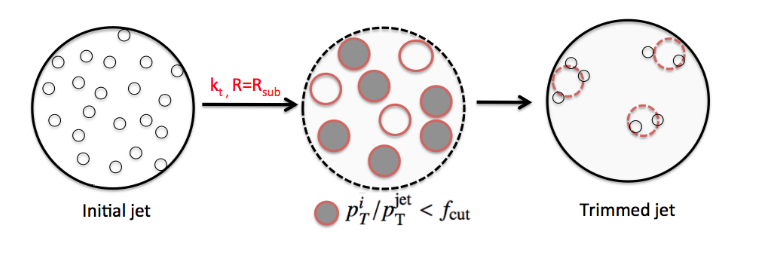
\includegraphics[width=0.9\textwidth]{jet_part/grooming/Figura_4.png}
  \caption{Schematic of the trimming algorithm.}
  \label{fig:trimming}
\end{figure}


\begin{figure}[!ht]
  \centering
      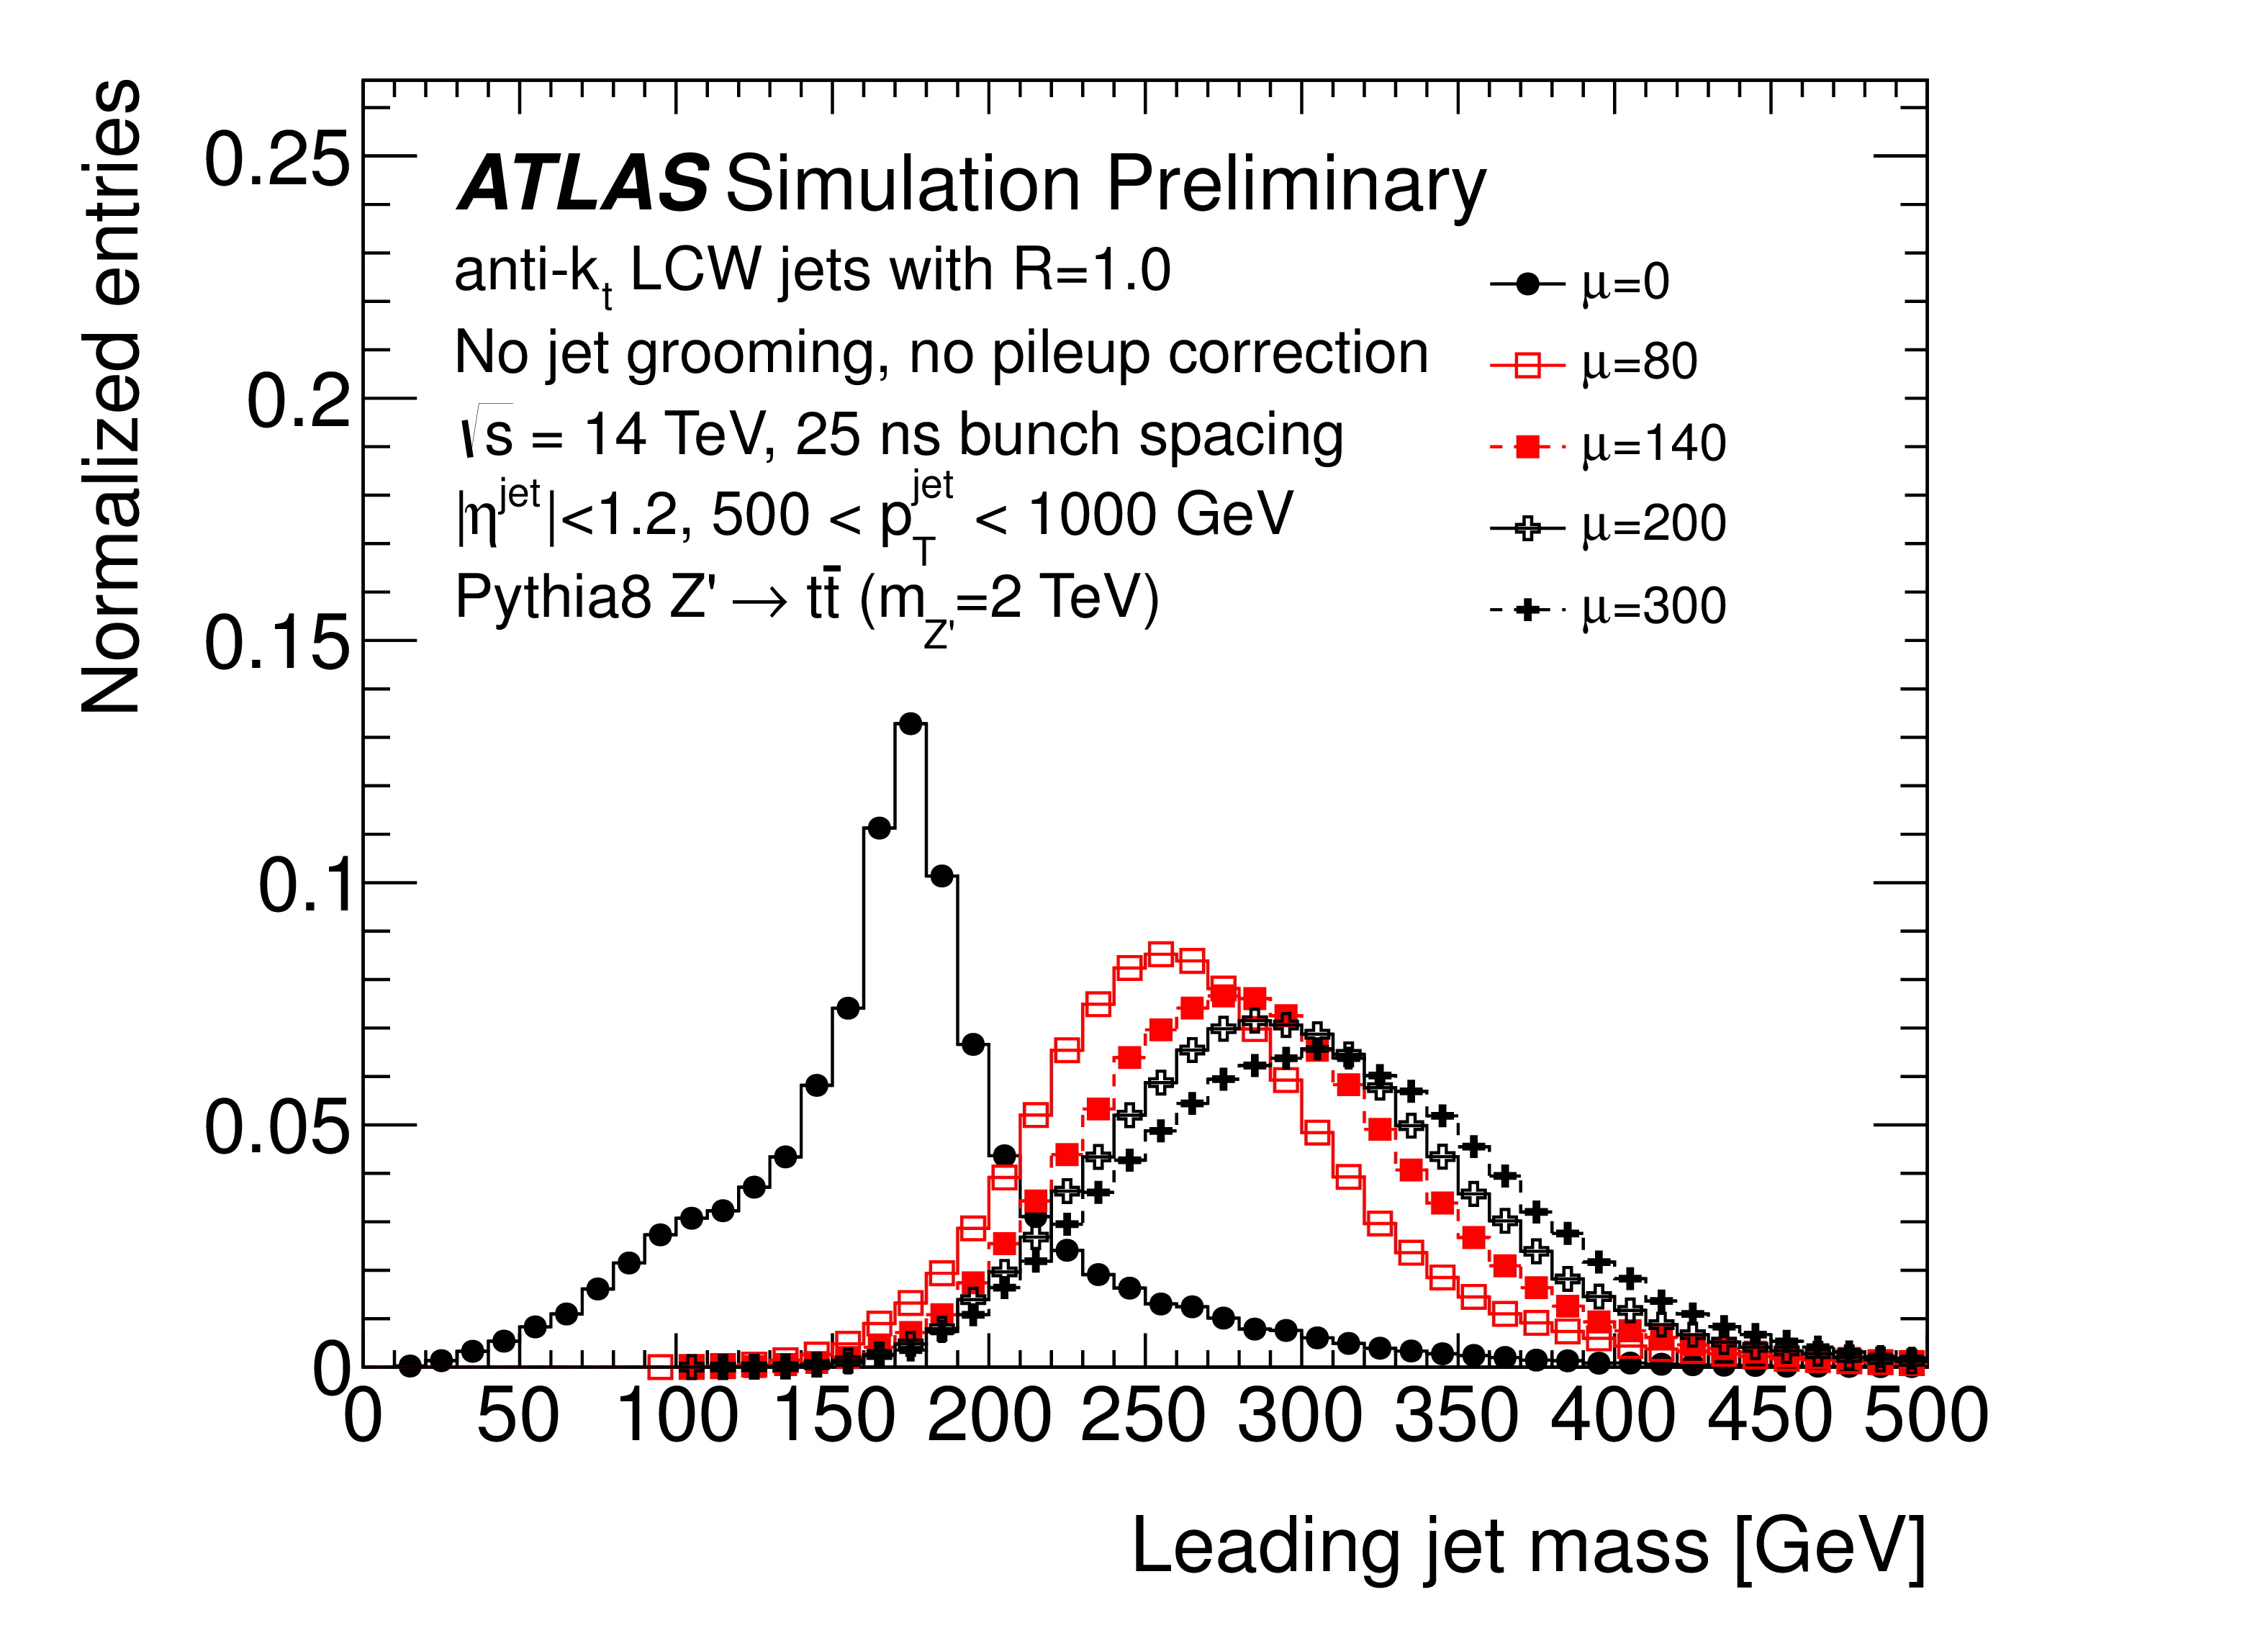
\includegraphics[width=0.5\textwidth]{jet_part/Jet_ungroomed_mass_pt_500.png}
  \caption[Effect of pile-up contamination]{Effect of pile-up contamination in large-$R$ jets: here shown different PU conditions parametrized by $\langle\mu\rangle$. From \cite{highlumi}.}
  \label{fig:largejetpu}
\end{figure}


\begin{figure}
    \centering
    \begin{subfigure}[b]{0.45\textwidth}
  \centering
        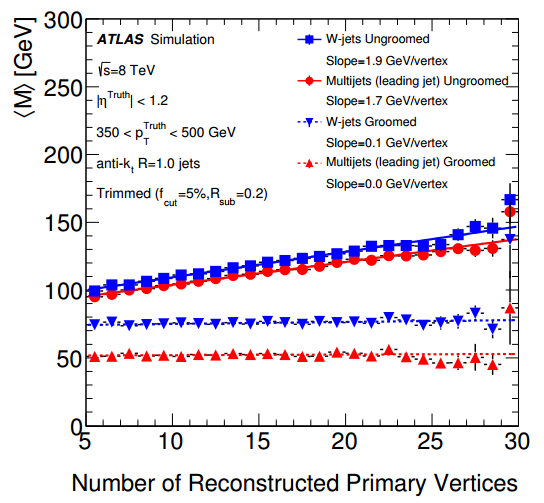
\includegraphics[width=0.78\textwidth]{jet_part/grooming/pileup.png}
 
%         \label{fig:gull}
    \end{subfigure}
    \begin{subfigure}[b]{0.45\textwidth}
  \centering
        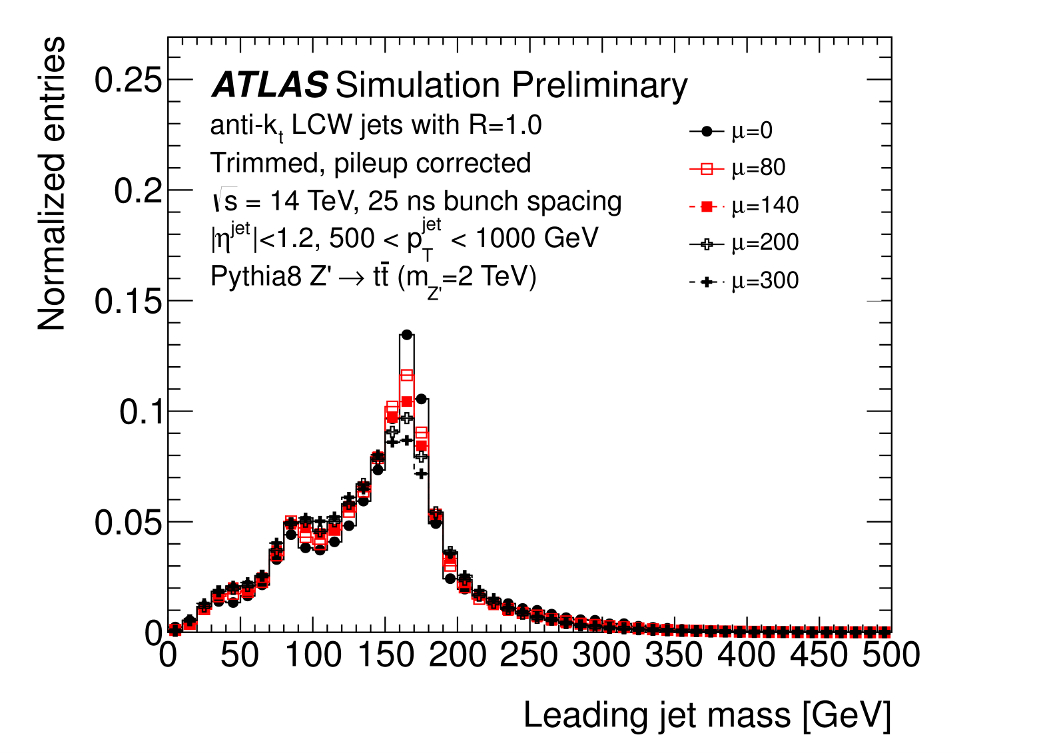
\includegraphics[width=\textwidth]{jet_part/Jet_pileupcorrected_mass_pt_500.jpeg}
   
%         \label{fig:tiger}
    \end{subfigure}
    \caption[Effect of pile-up before and after trimming]{Left: mass reconstructed as a function of the number of primary vertices (parameterizing PU) for different samples; after trimming procedure the mass is pretty much independent of PU for all the samples. Right: mass distributions for different PU conditions: after trimming the reconstruction is not degraded as much as Figure \ref{fig:largejetpu}.} 
    \label{fig:trimmingperformance}
\end{figure}


\section{Tracks details}\label{sec:tracking}
The requirements applied on the track used in the work presented in this note are given here:
\begin{itemize}
 \item $p_T^{track} > 400$ MeV;
 \item $|\eta|<$ 2.5;
 \item Maximum 7 hits in the Pixel and STC sub-detectors;
 \item Maximum 1 Pixel hole;
 \item Maximum 2 silicon holes;
 \item Less than 3 shared modules;
 \item Maximum 2 mm of displacement along beam axis ($z_0$) from the primary vertex;
 \item Maximum 2.5 mm of distance in x-y plane from the primary vertex and point of closest approach ($d_0$).
\end{itemize}

\section{Alternative Performance Figure of Merit (FoM)}

A concrete, quantitative feature has to be defined in order to understand which observable is ``better'', in the sense that we would prefer one or the other according to this criterion. This is often referred to as \textit{Figure of Merit} or simply FoM.

There are few ways to look at the FoM: one can e.g. na\"ively think about the mean of the mass distribution, since closer values of the mean to the e.g. $W$ or $Z$ mass (if we are speaking about $W/Z$ decays) indicate a more correct mass reconstruction. However, this does not take into account the width of this distribution, as a large width spoils the reconstruction in terms of percentage of jets misreconstructed. Moreover, the mean is not as important since it can be rescaled to the desired value in a calibration procedure.

\subsection{Gaussian Fit}

The important feature to keep in mind, in fact, is the underlying physics which brings us to calculate the mass of a jet. In figure \ref{fig:search} this is made clear: if the width of the invariant mass distribution of the jet is smaller (highlighted), it allows a bigger background rejection, here shown as the QCD dijet, for the same signal efficiency, by means of a simple mass requirement.

\begin{figure}[!ht]
  \centering
      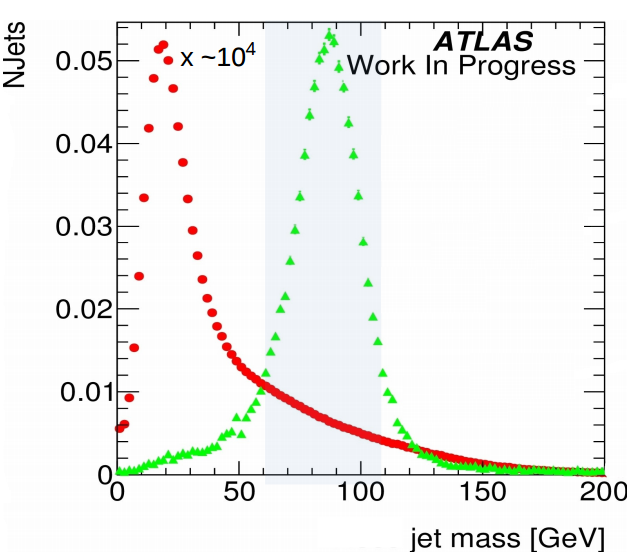
\includegraphics[width=0.55\textwidth]{jet_part/search.png}
  \caption[QCD and $W'$ mass distribution]{Mass distributions: in red the QCD dijet background rescaled, in green the $W/Z$ from the $W'$ sample. Highlighted the width of the 68\% of the $W/Z$ distribution.}
  \label{fig:search}
\end{figure}

The width $\sigma$ of the distribution, which can be obtained from a fit to the Gaussian core, is already a valid FoM, which has an underlying physical feature. Moreover, in order to be independent from the mean of the distribution, the width can be divided by the mean itself.
This was in fact the FoM which was used at the beginning of the work for this thesis, since it provided a simple and fast solution. However, special care must be used both in the procedure of fitting Gaussian cores of responses, since they are asymmetric, and to how the tails are treated.

\begin{figure}[!ht]
  \centering
      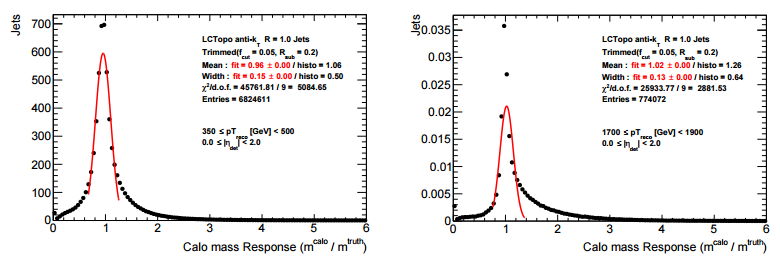
\includegraphics[width=0.9\textwidth]{jet_part/wrongsigma.png}
  \caption[Gaussian fit for QCD multijet]{Mass Response distributions for the QCD multijet for various $\pt$ ranges: on the right the failure of the Gaussian fit shows the limitation of this approach to serve as the Figure of Merit. On the plot the fit parameters and transverse momentum ranges.}
  \label{fig:wrongsigma32}
\end{figure}

The situation is depicted e.g. in Figure \ref{fig:wrongsigma32}, where a mass response is shown for calorimeter mass for QCD multijet: here the presence of a right-handed tail which enhances going from low to high transverse momenta makes the Gaussian fit clearly not the tool which provides the stability needed. The ideal tool should consider the presence of at least tails outside the Gaussian core and should converge to the intuition of the standard deviation for a perfect Gaussian distribution.
The closest tool to this idea was found to be the \textit{InterQuantile Range}, which is presented in the body of this note.


\section{Kinematic distributions of signal and background samples}\label{sec:kinematic}
Kinematic distributions for all the samples, $\pt$ $\eta$ and $\phi$ are shown.

\begin{figure}
    \centering
    \begin{subfigure}[b]{0.45\textwidth}
        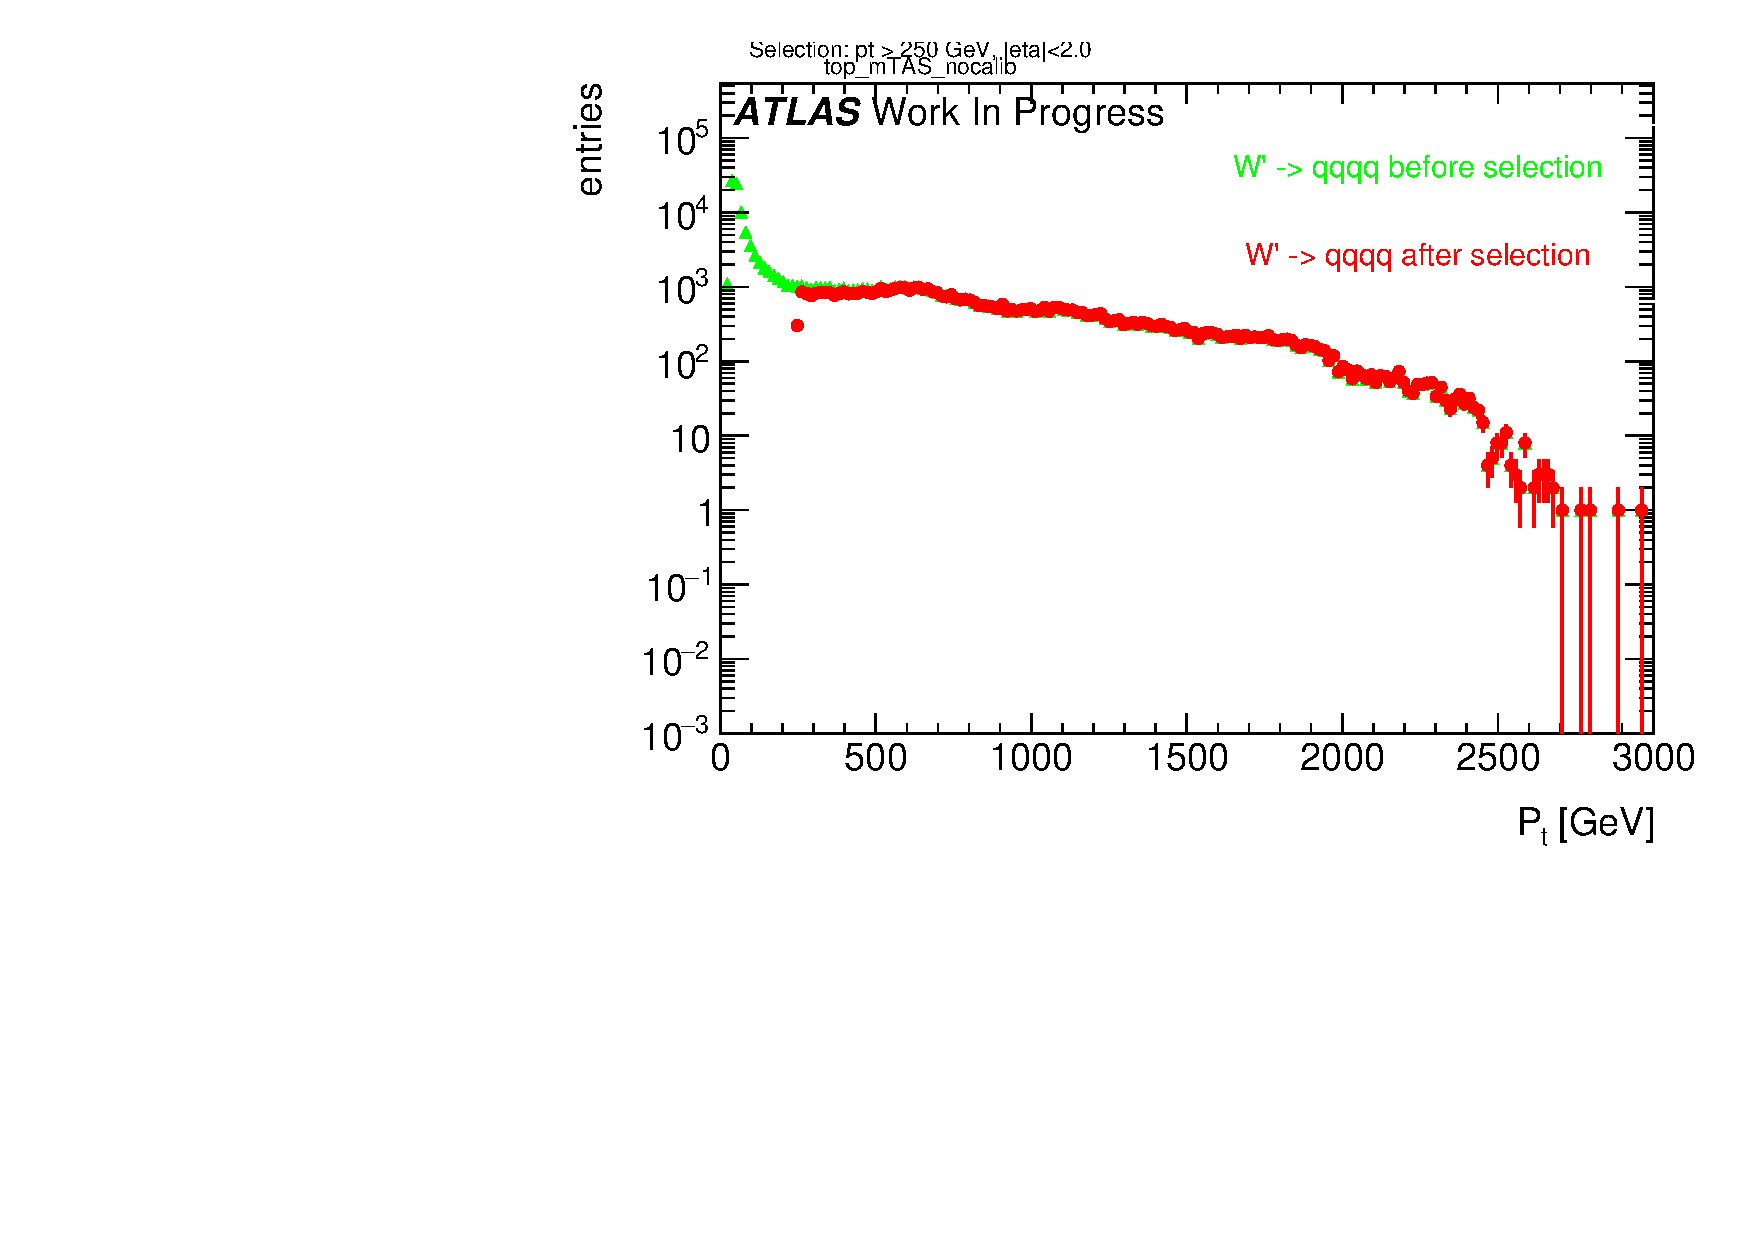
\includegraphics[width=\textwidth]{jet_part/appendixA/tops/1cfrt_h_FatJet_pt.pdf}
        \caption{$\pt$ distribution}
        \label{fig:gull}
    \end{subfigure}
    \begin{subfigure}[b]{0.45\textwidth}
        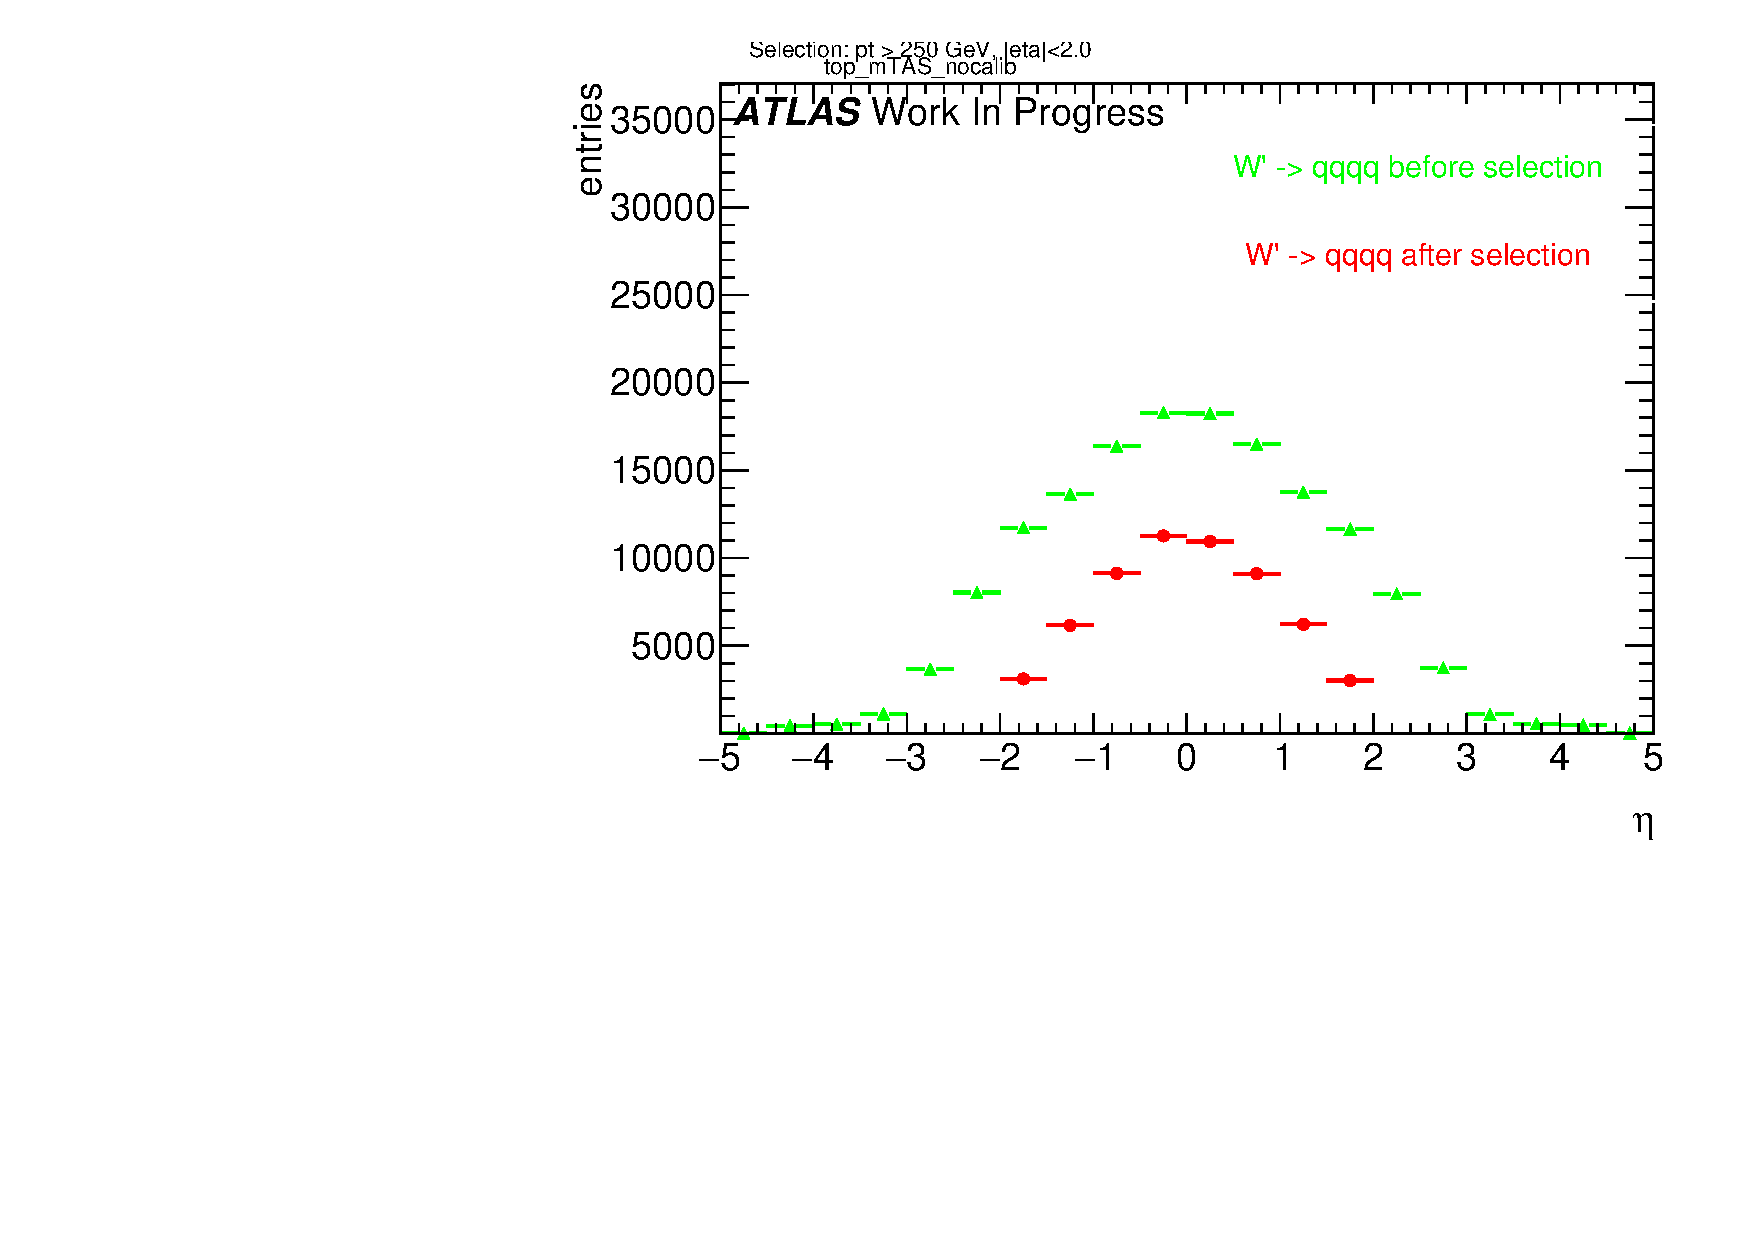
\includegraphics[width=\textwidth]{jet_part/appendixA/tops/1cfrt_h_FatJet_eta.pdf}
        \caption{$\eta$ distribution}
        \label{fig:tiger}
    \end{subfigure}
    \begin{subfigure}[b]{0.45\textwidth}
        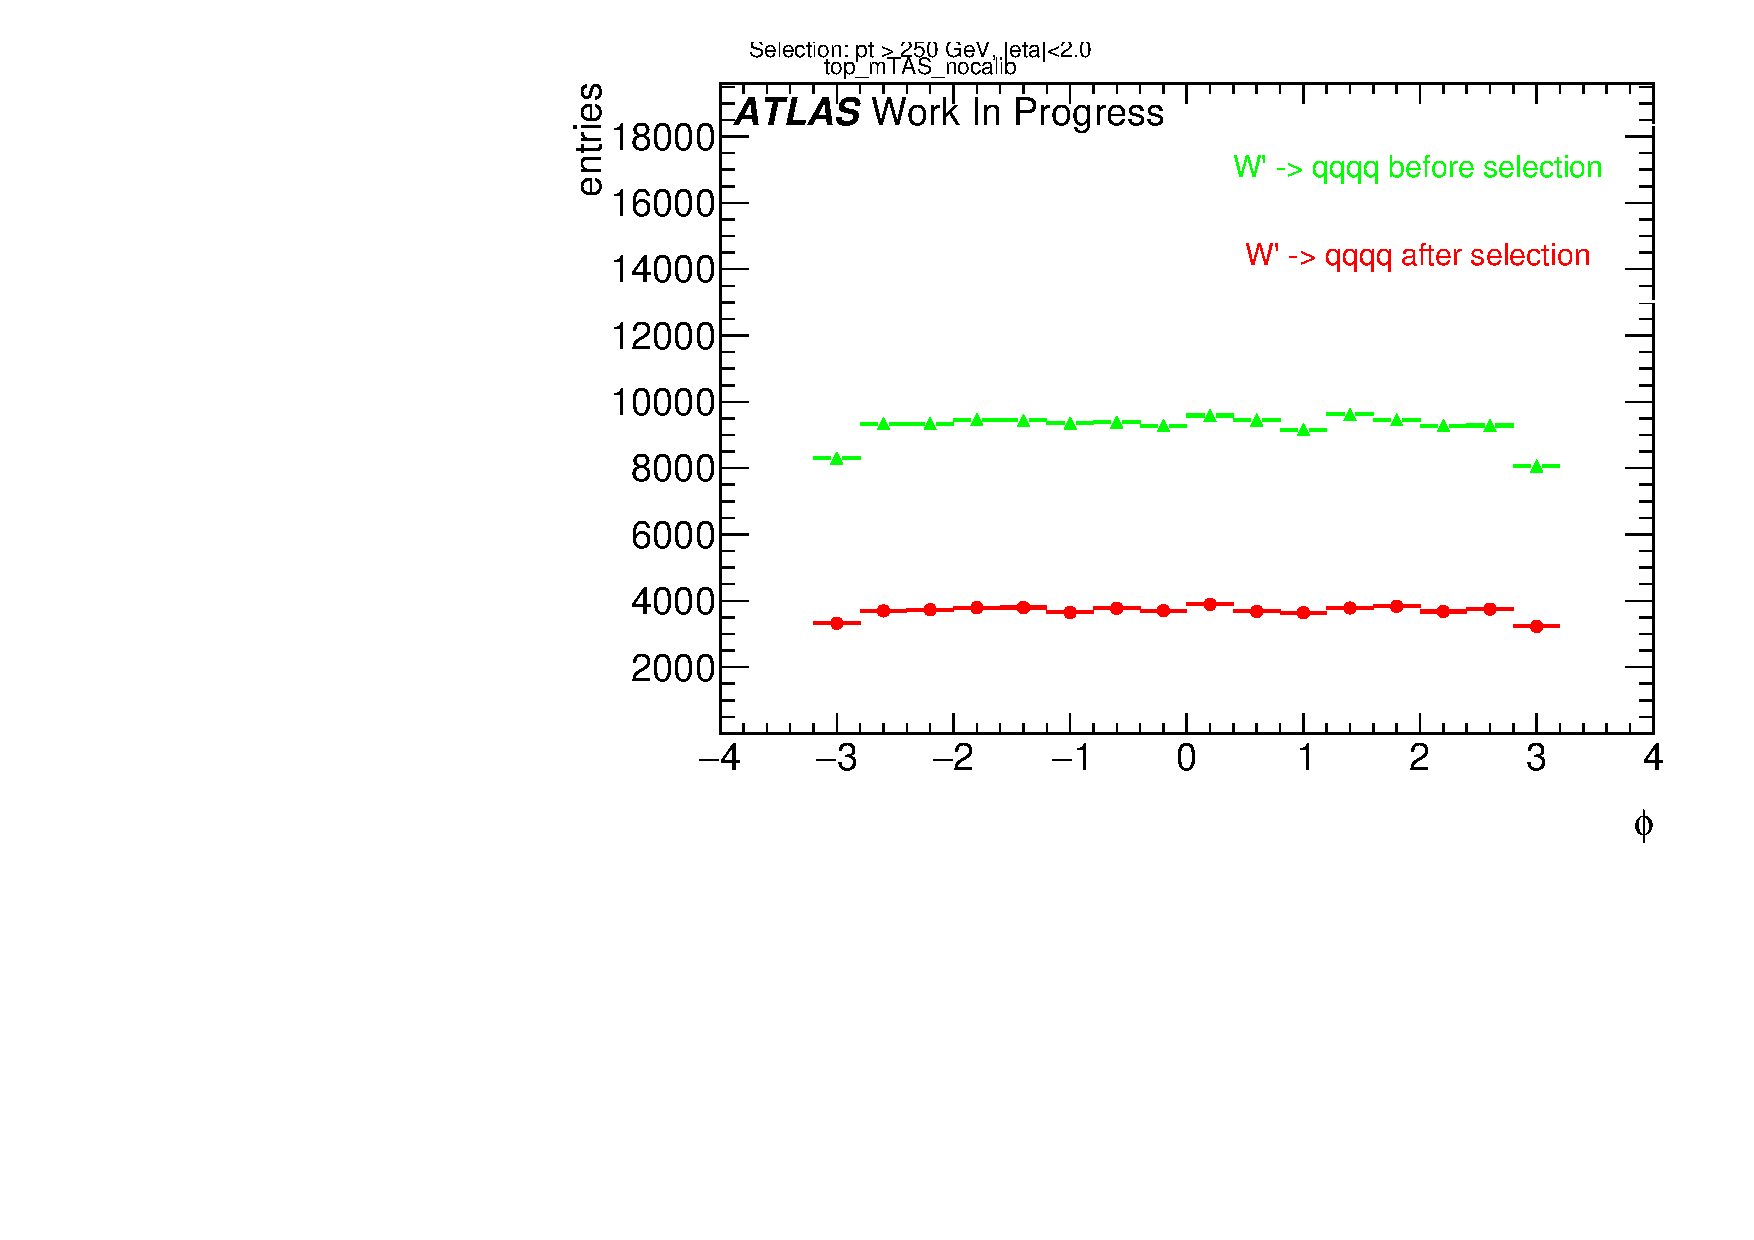
\includegraphics[width=\textwidth]{jet_part/appendixA/tops/1cfrt_h_FatJet_psi.pdf}
        \caption{$\phi$ distribution}
        \label{fig:mouse}
    \end{subfigure}
    \caption{Boosted tops kinematic distribution.}\label{fig:animals}
\end{figure}


\begin{figure}
    \centering
    \begin{subfigure}[b]{0.45\textwidth}
        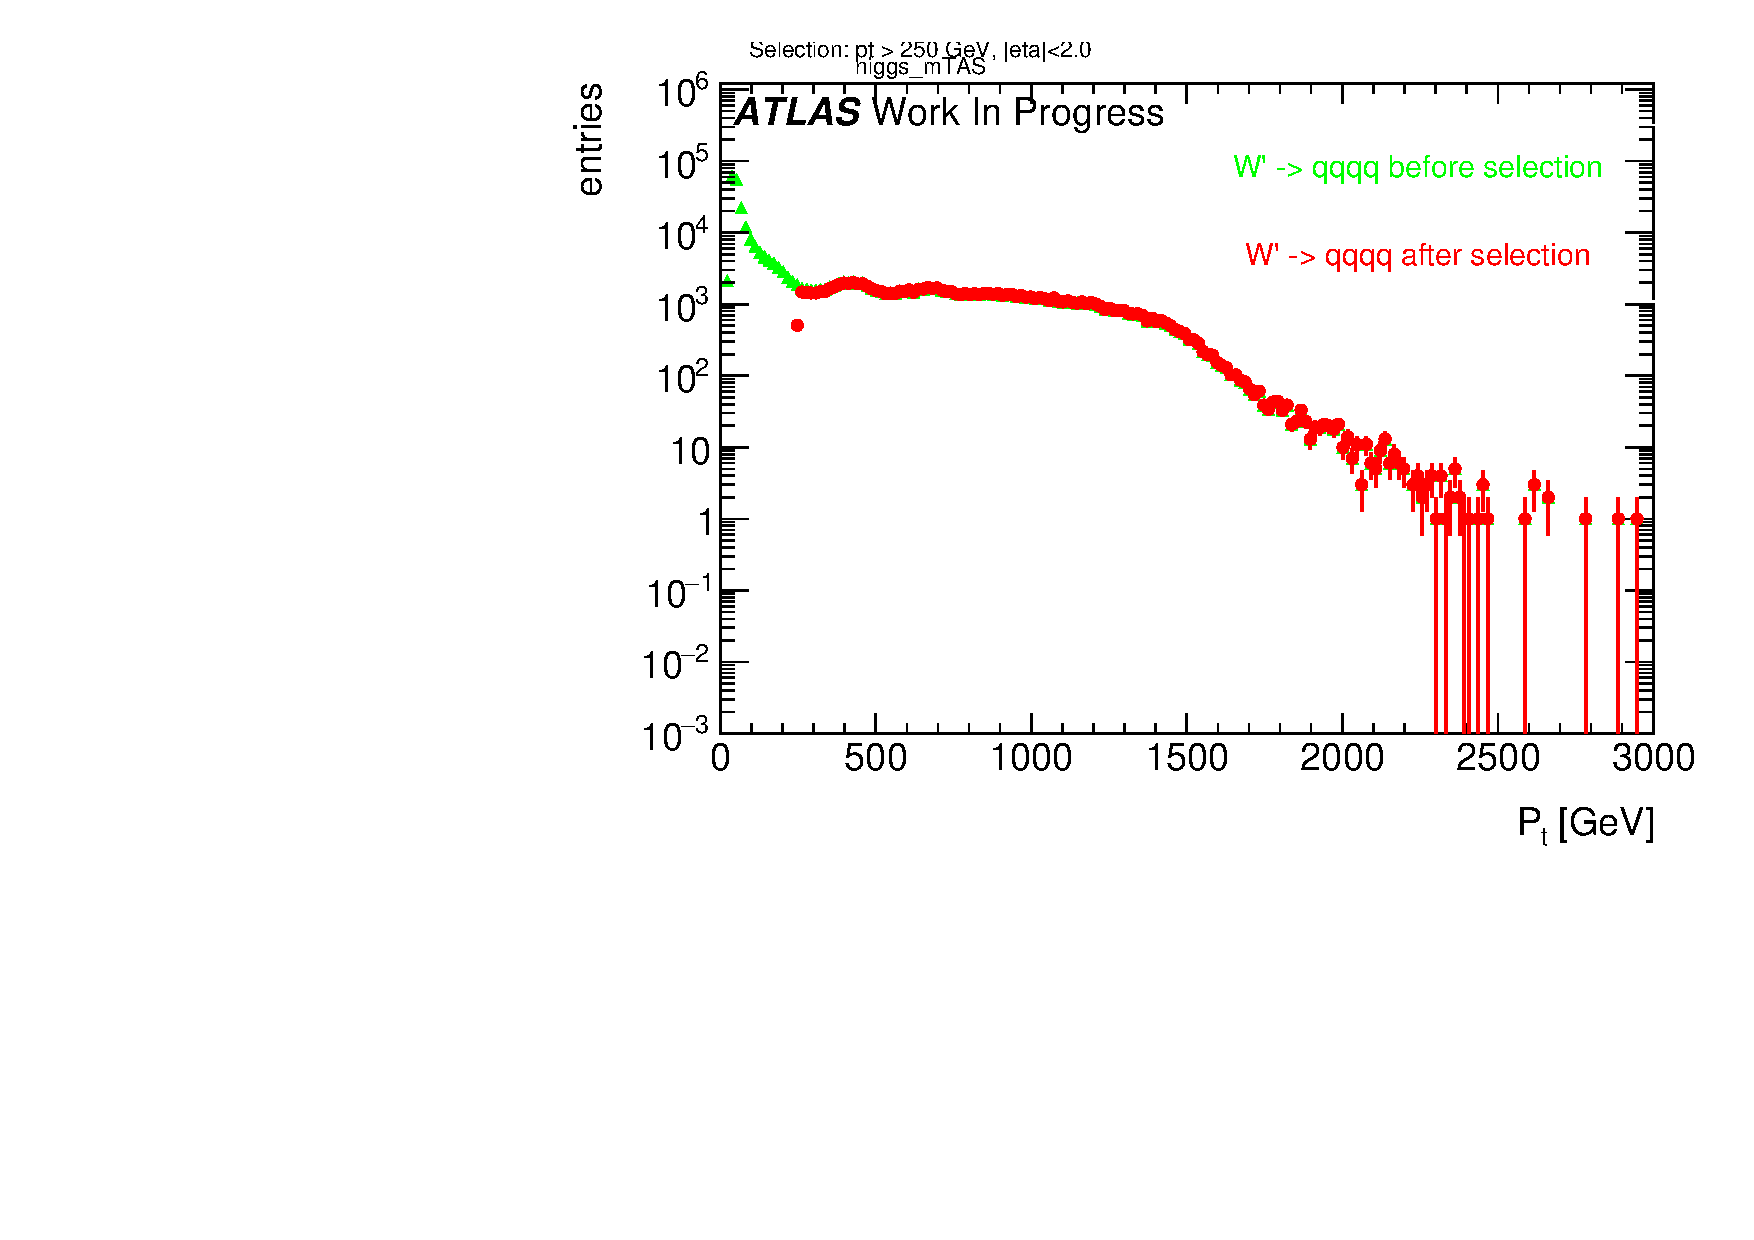
\includegraphics[width=\textwidth]{jet_part/appendixA/higgs/1cfrt_h_FatJet_pt.pdf}
        \caption{$\pt$ distribution}
        \label{fig:gull}
    \end{subfigure}
    \begin{subfigure}[b]{0.45\textwidth}
        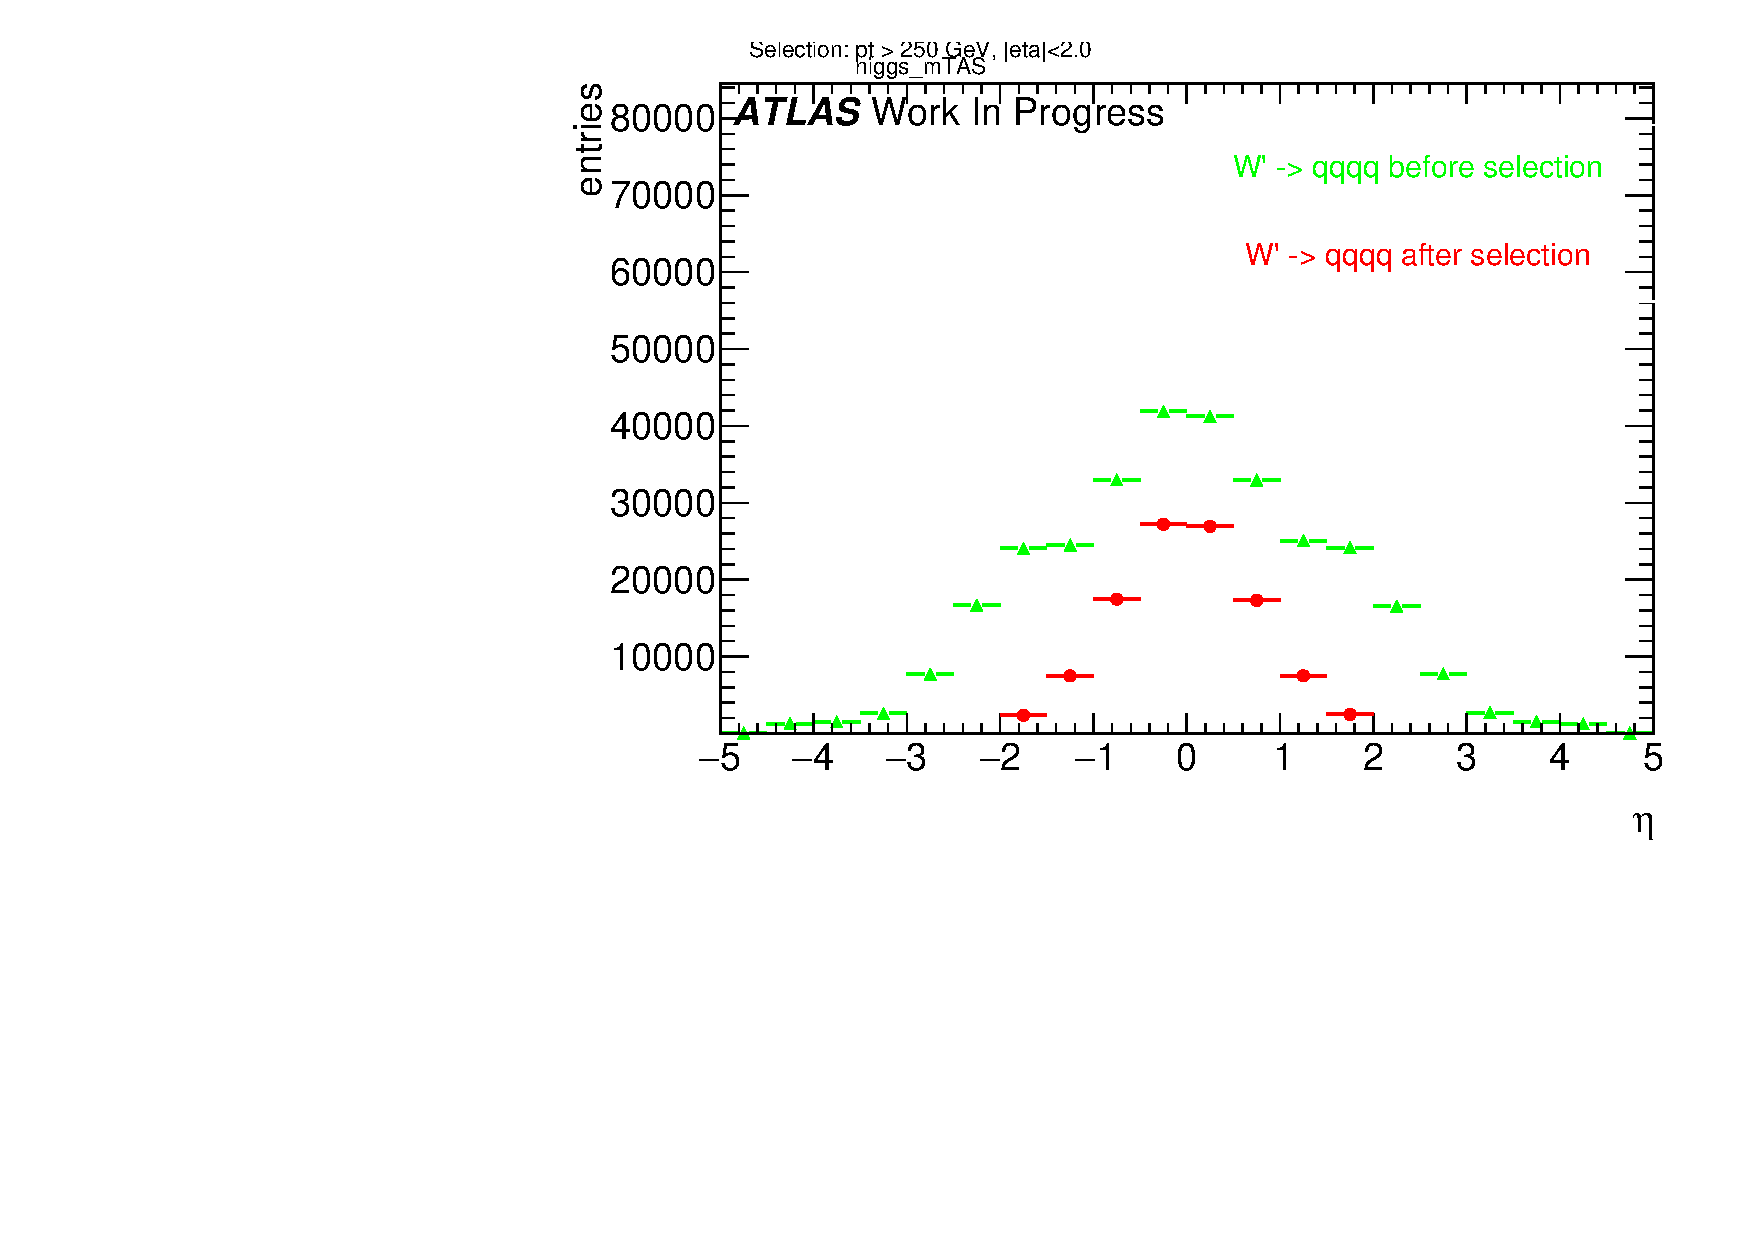
\includegraphics[width=\textwidth]{jet_part/appendixA/higgs/1cfrt_h_FatJet_eta.pdf}
        \caption{$\eta$ distribution}
        \label{fig:tiger}
    \end{subfigure}
    \begin{subfigure}[b]{0.45\textwidth}
        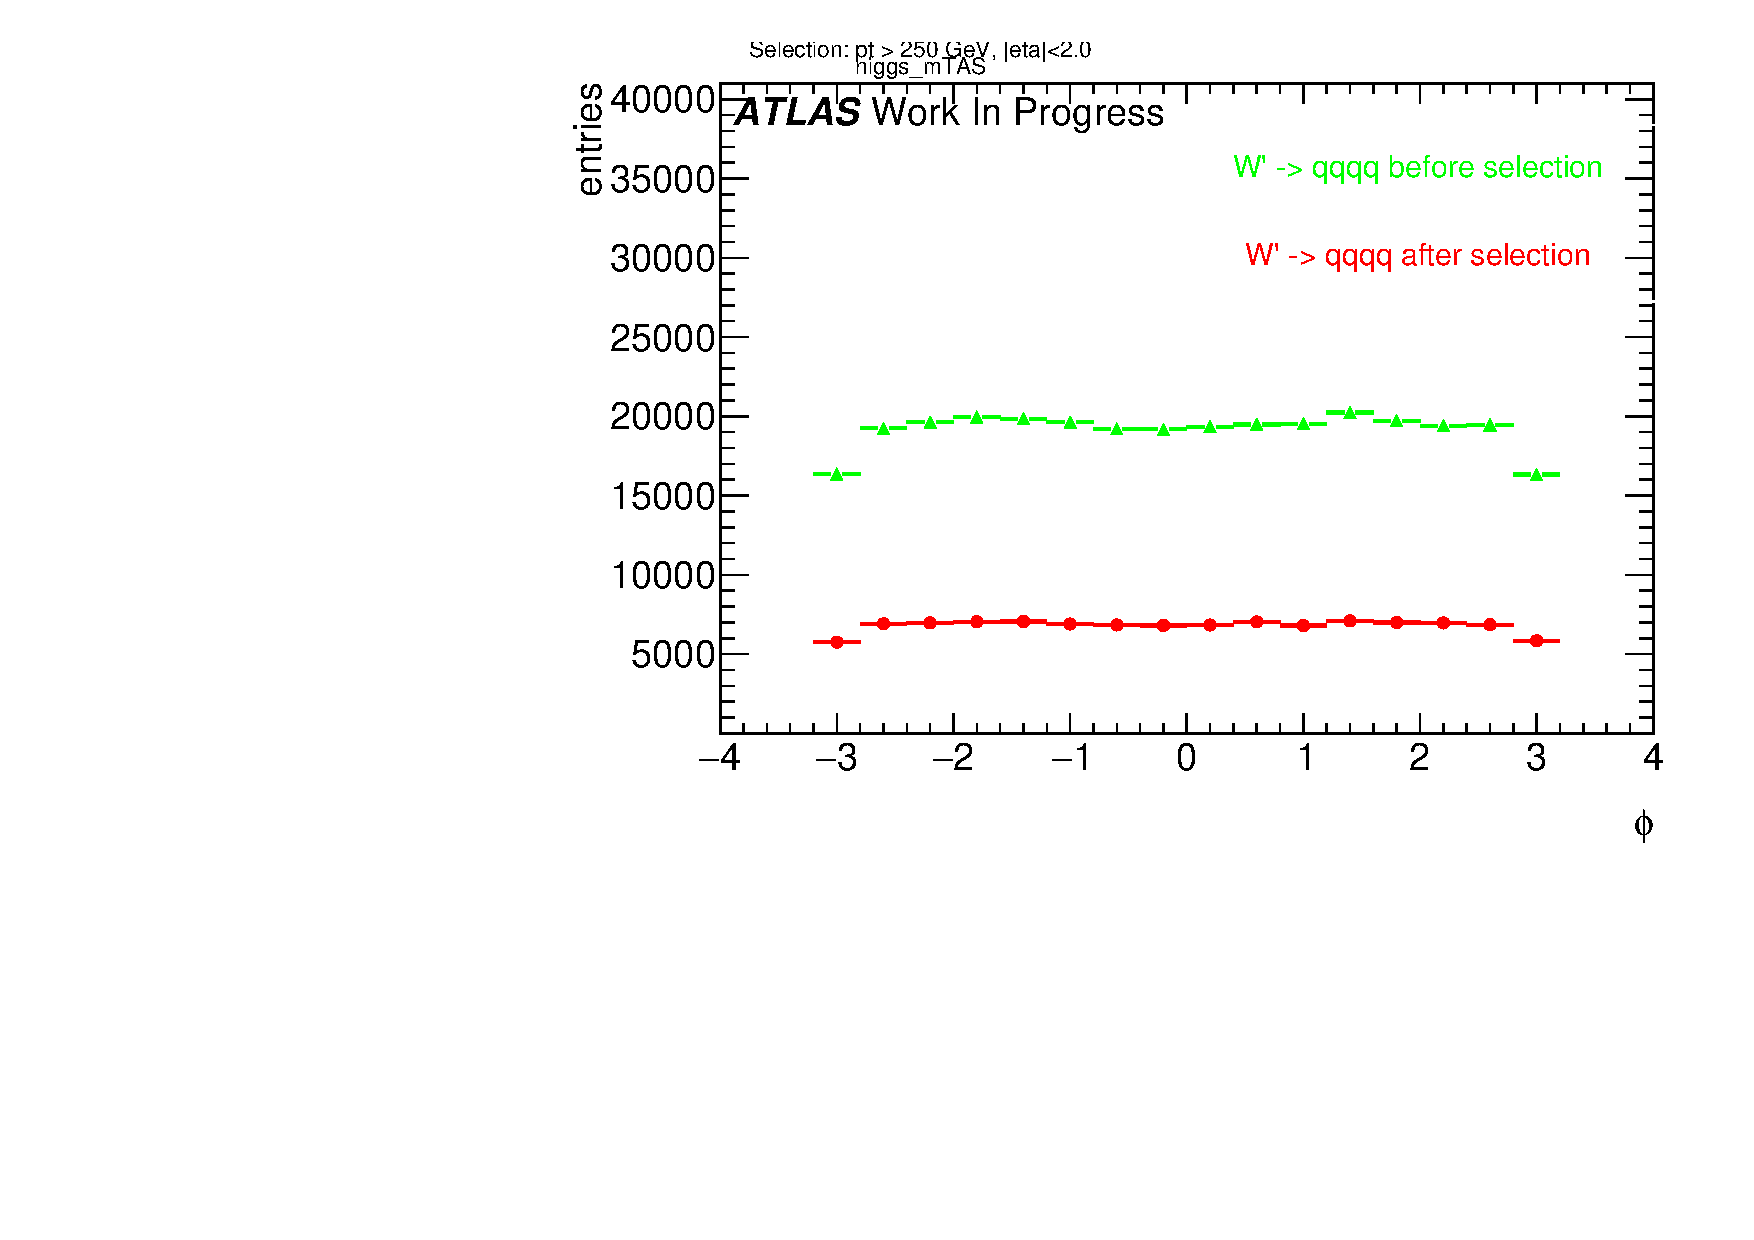
\includegraphics[width=\textwidth]{jet_part/appendixA/higgs/1cfrt_h_FatJet_psi.pdf}
        \caption{$\phi$ distribution}
        \label{fig:mouse}
    \end{subfigure}
    \caption{RS-Graviton kinematic distribution.}\label{fig:animals}
\end{figure}

\begin{figure}
    \centering
   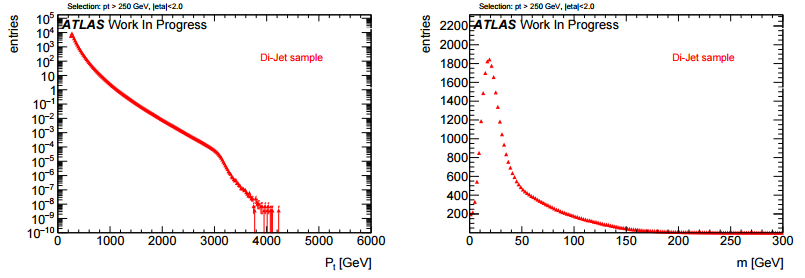
\includegraphics[width=\textwidth]{jet_part/appendixA/qcd/qcdkinematics.png}
   
    \caption{QCD dijet transverse momentum and mass distributions.}
    \label{fig:qcdkinematics}
\end{figure}

\begin{figure}[!ht]
  \centering
      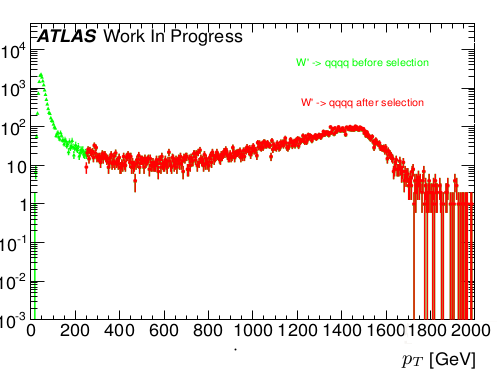
\includegraphics[width=0.5\textwidth]{jet_part/ptjcobian.png}
  \caption{The $\pt$ distribution of a 3 TeV resonance from the hadronically decaying $W$ or $Z$, in logarithmic plot. As can be seen, the jacobian peak is around $\pt\simeq m_{W'}/2\simeq 1.5$ TeV.}
  \label{fig:ptjacobian}
\end{figure}


\begin{figure}
    \centering
    \begin{subfigure}[b]{0.45\textwidth}
	\centering
        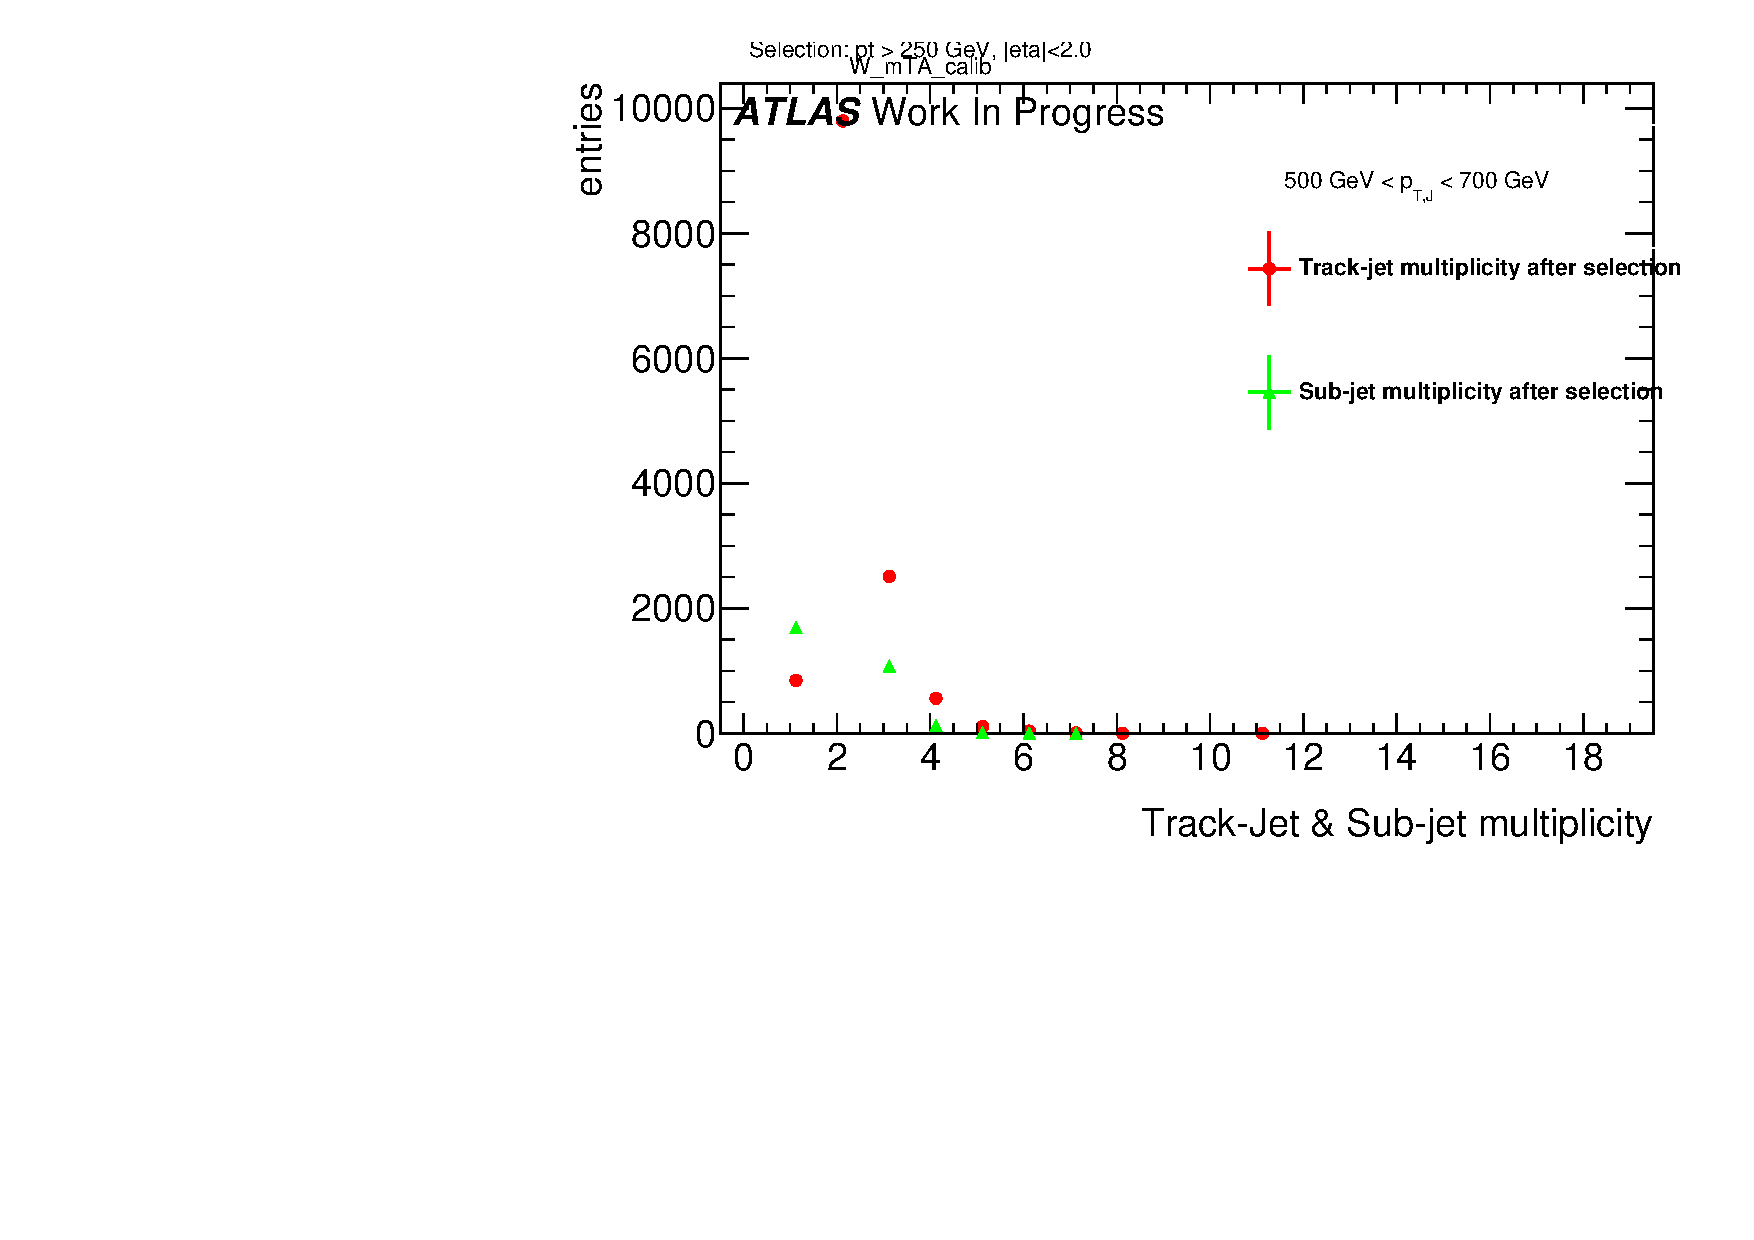
\includegraphics[width=\textwidth]{jet_part/mta/13cfrt_h_SubJet_aftersel_ptJ03TAmult.pdf}
 
%         \label{fig:gull}
    \end{subfigure}
    \begin{subfigure}[b]{0.45\textwidth}
	\centering
        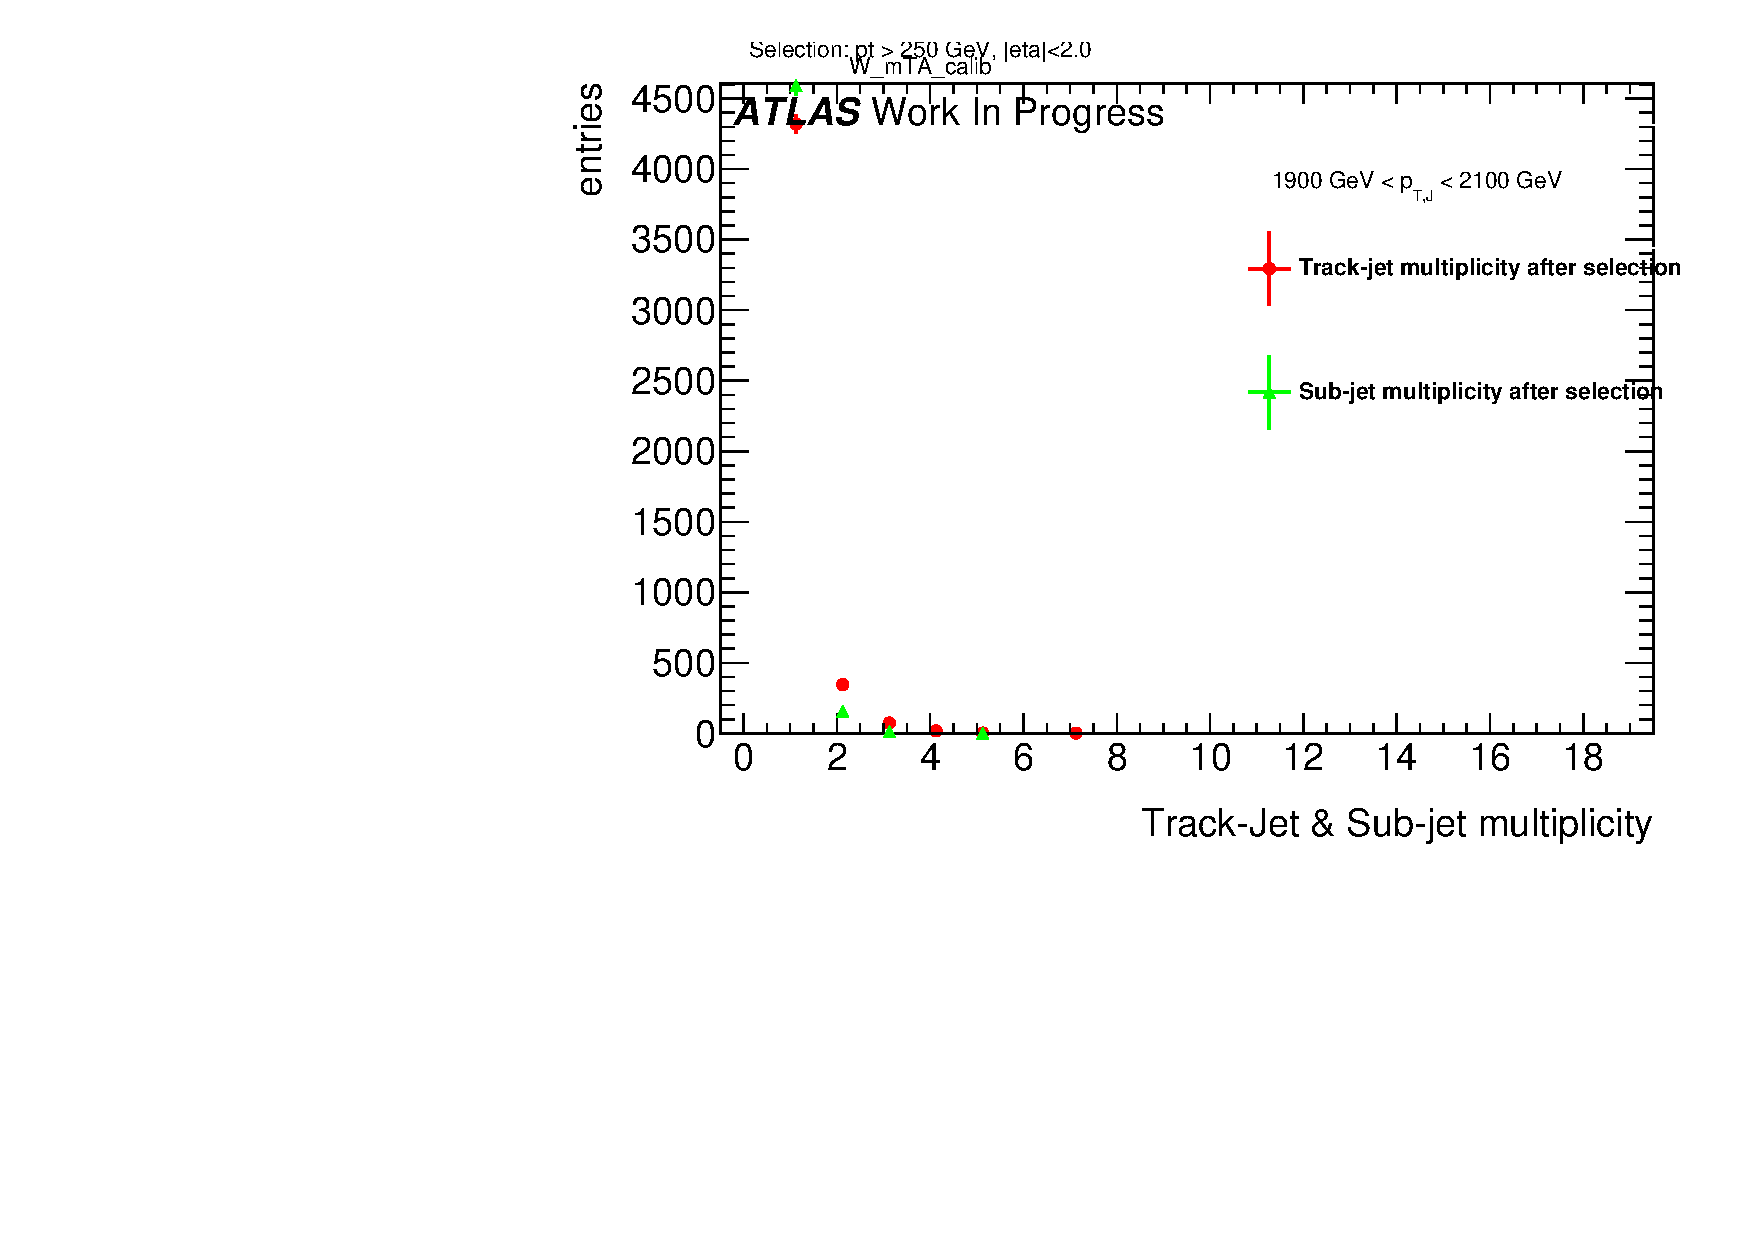
\includegraphics[width=\textwidth]{jet_part/mta/13cfrt_h_SubJet_aftersel_ptJ10TAmult.pdf}
   
%         \label{fig:tiger}
    \end{subfigure}
    \caption{Sub-jet and Track-jet (jets created having tracks as input) multiplicity, for selected bins of transverse momentum.} 
    \label{fig:multi}
\end{figure}


% \begin{figure}
%     \centering
%    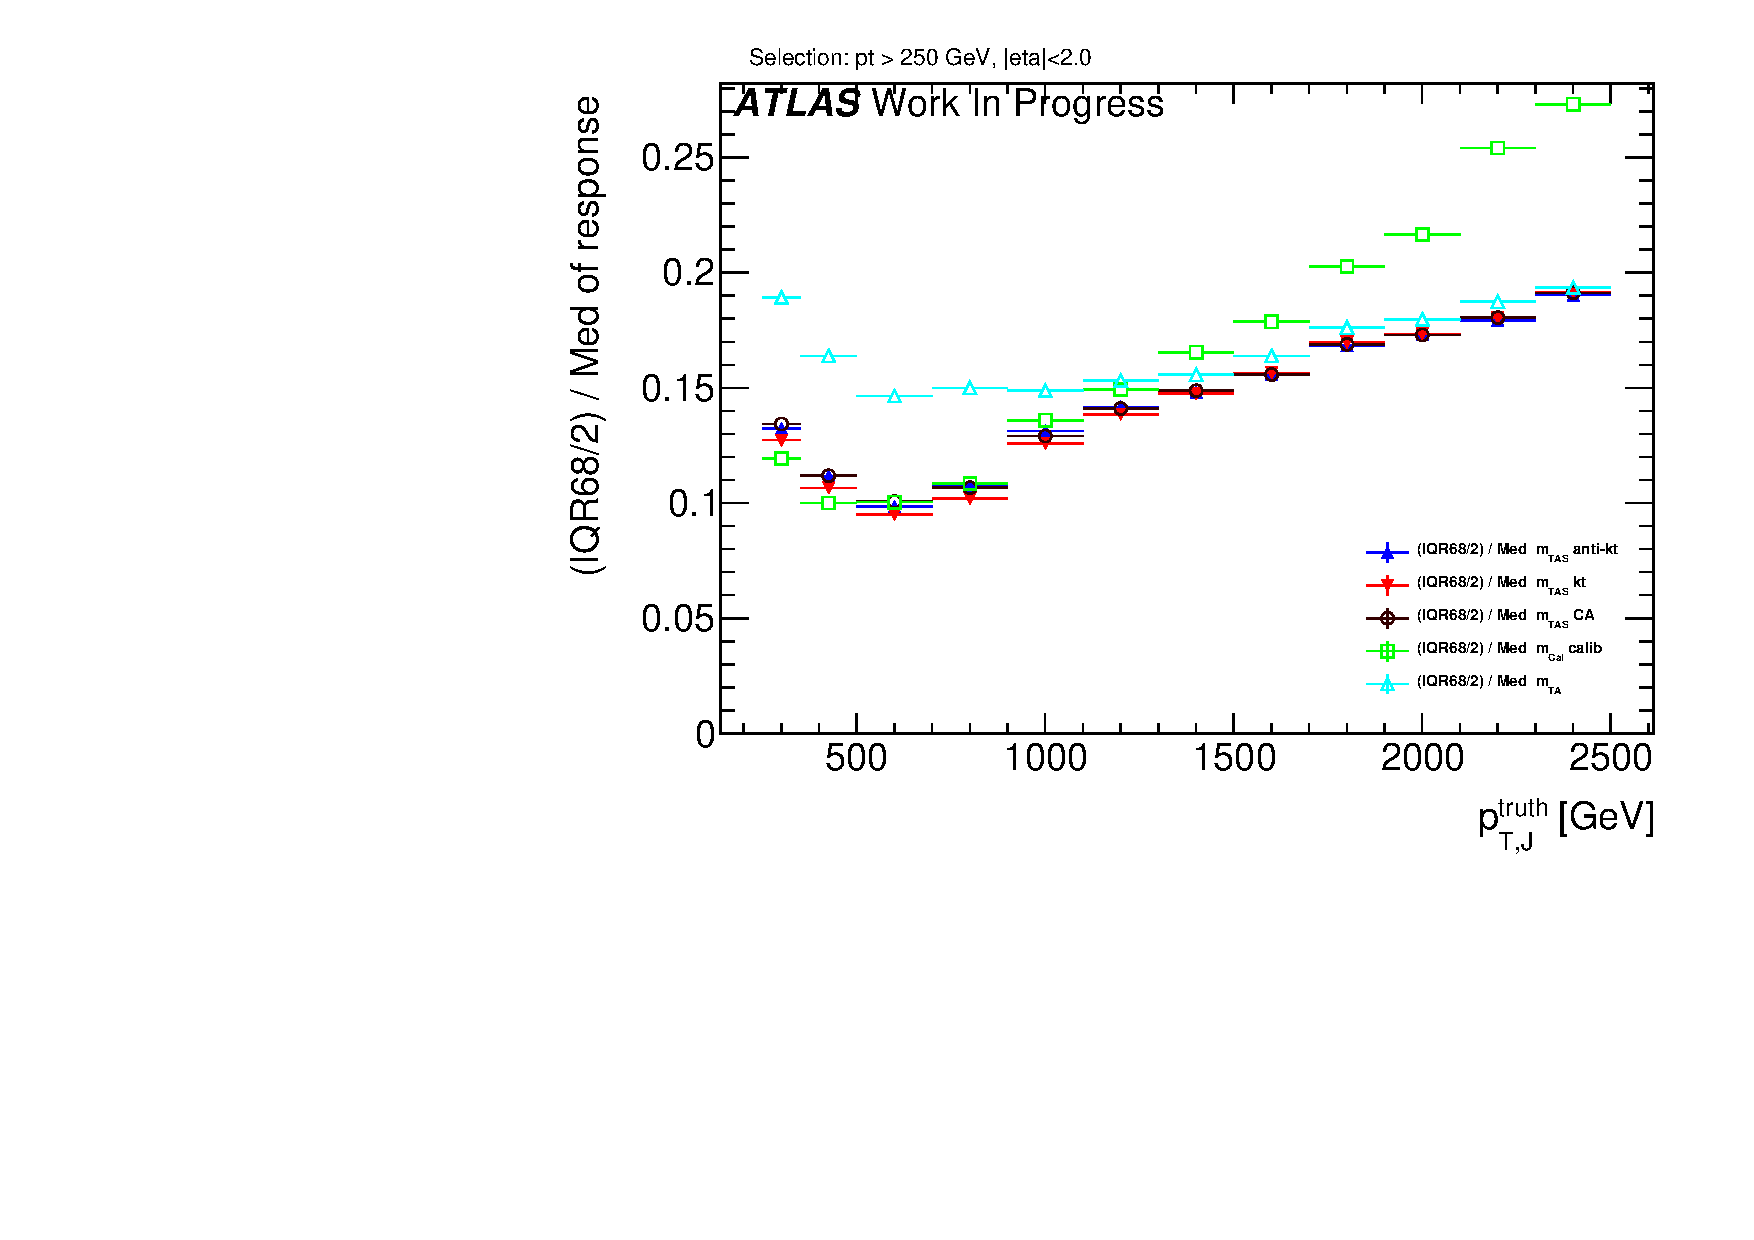
\includegraphics[width=\textwidth]{jet_part/mtas/71graphcftr_h_JetRatio_mJ12CALOIQRoM_Wprime_Allalgos.pdf}
   
%     \caption{Performance of $\mtas$ with different reclustering algorithm for the sub-jets: anti-k$_t$, k$_t$ and C/A. Boosted $W/Z$ sample.}
%     \label{fig:allalgow}
% \end{figure}

% \begin{figure}
%     \centering
%    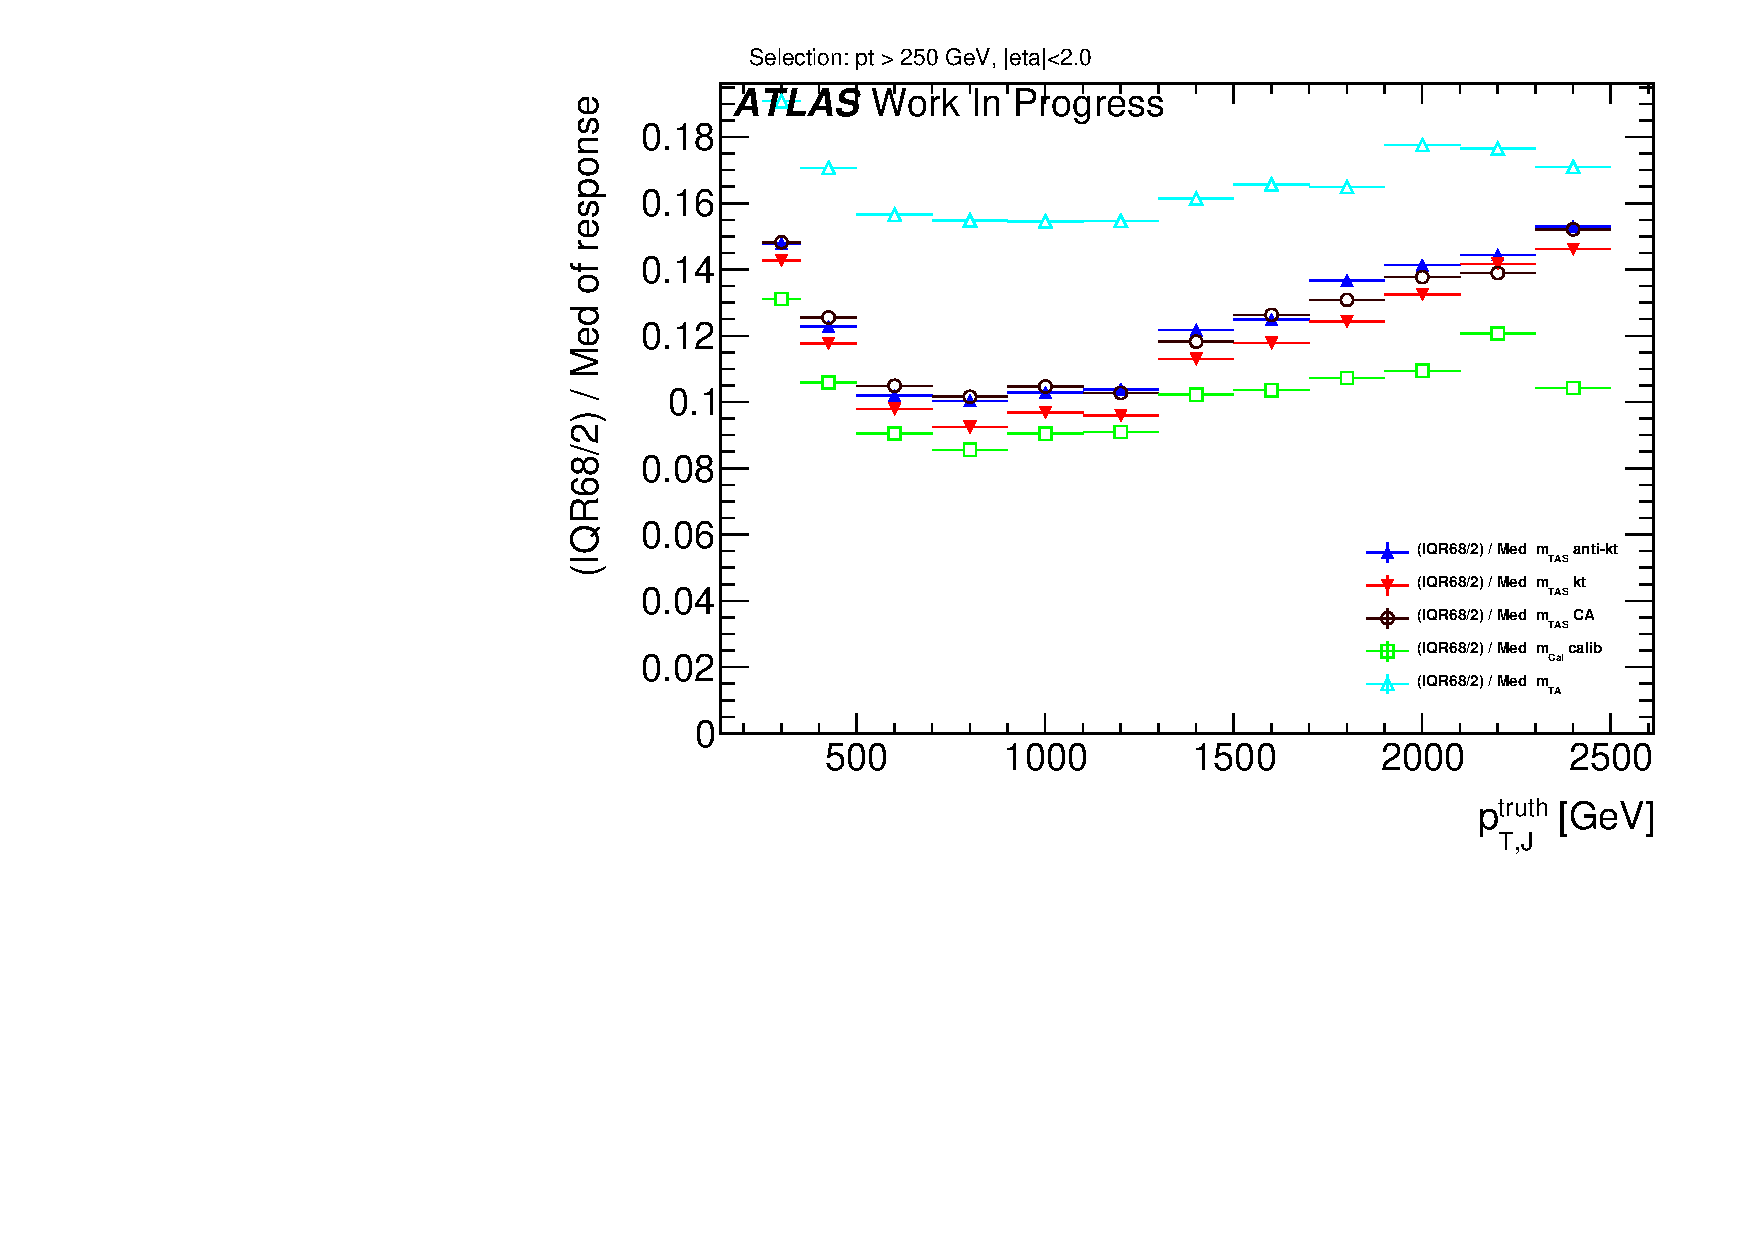
\includegraphics[width=\textwidth]{jet_part/mtas/71graphcftr_h_JetRatio_mJ12CALOTopsCalib.pdf}
   
%     \caption{Performance of $\mtas$ with different reclustering algorithm for the sub-jets: anti-k$_t$, k$_t$ and C/A. Boosted top sample.}
%     \label{fig:allalgotop}
% \end{figure}

% \begin{figure}
%     \centering
%    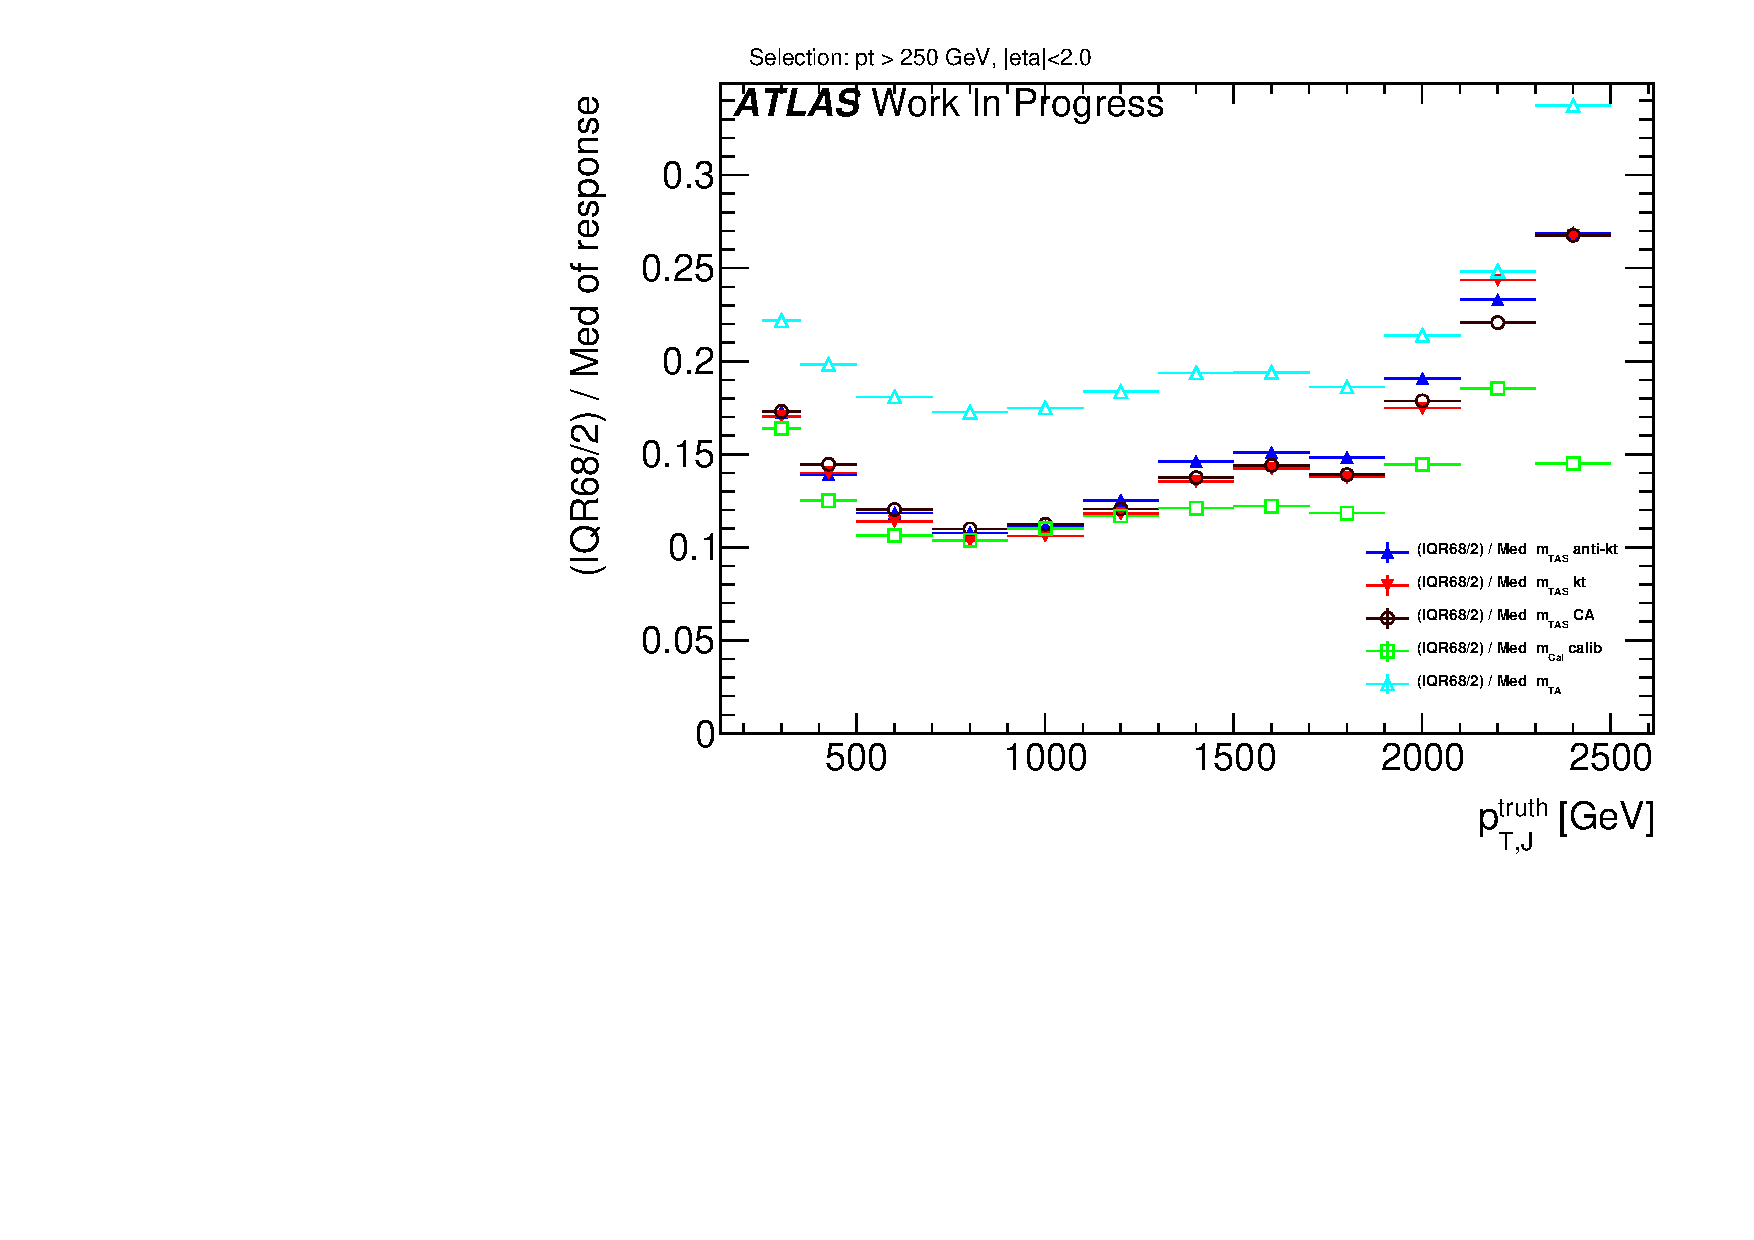
\includegraphics[width=\textwidth]{jet_part/mtas/71graphcftr_h_JetRatio_mJ12CALOIQRoMHiggsNOCalib.pdf}
   
%     \caption{Performance of $\mtas$ with different reclustering algorithm for the sub-jets: anti-k$_t$, k$_t$ and C/A. Boosted higgs sample.}
%     \label{fig:allalgohiggs}
% \end{figure}


\begin{figure}
    \centering
    \begin{subfigure}[b]{0.5\textwidth}
	\centering
        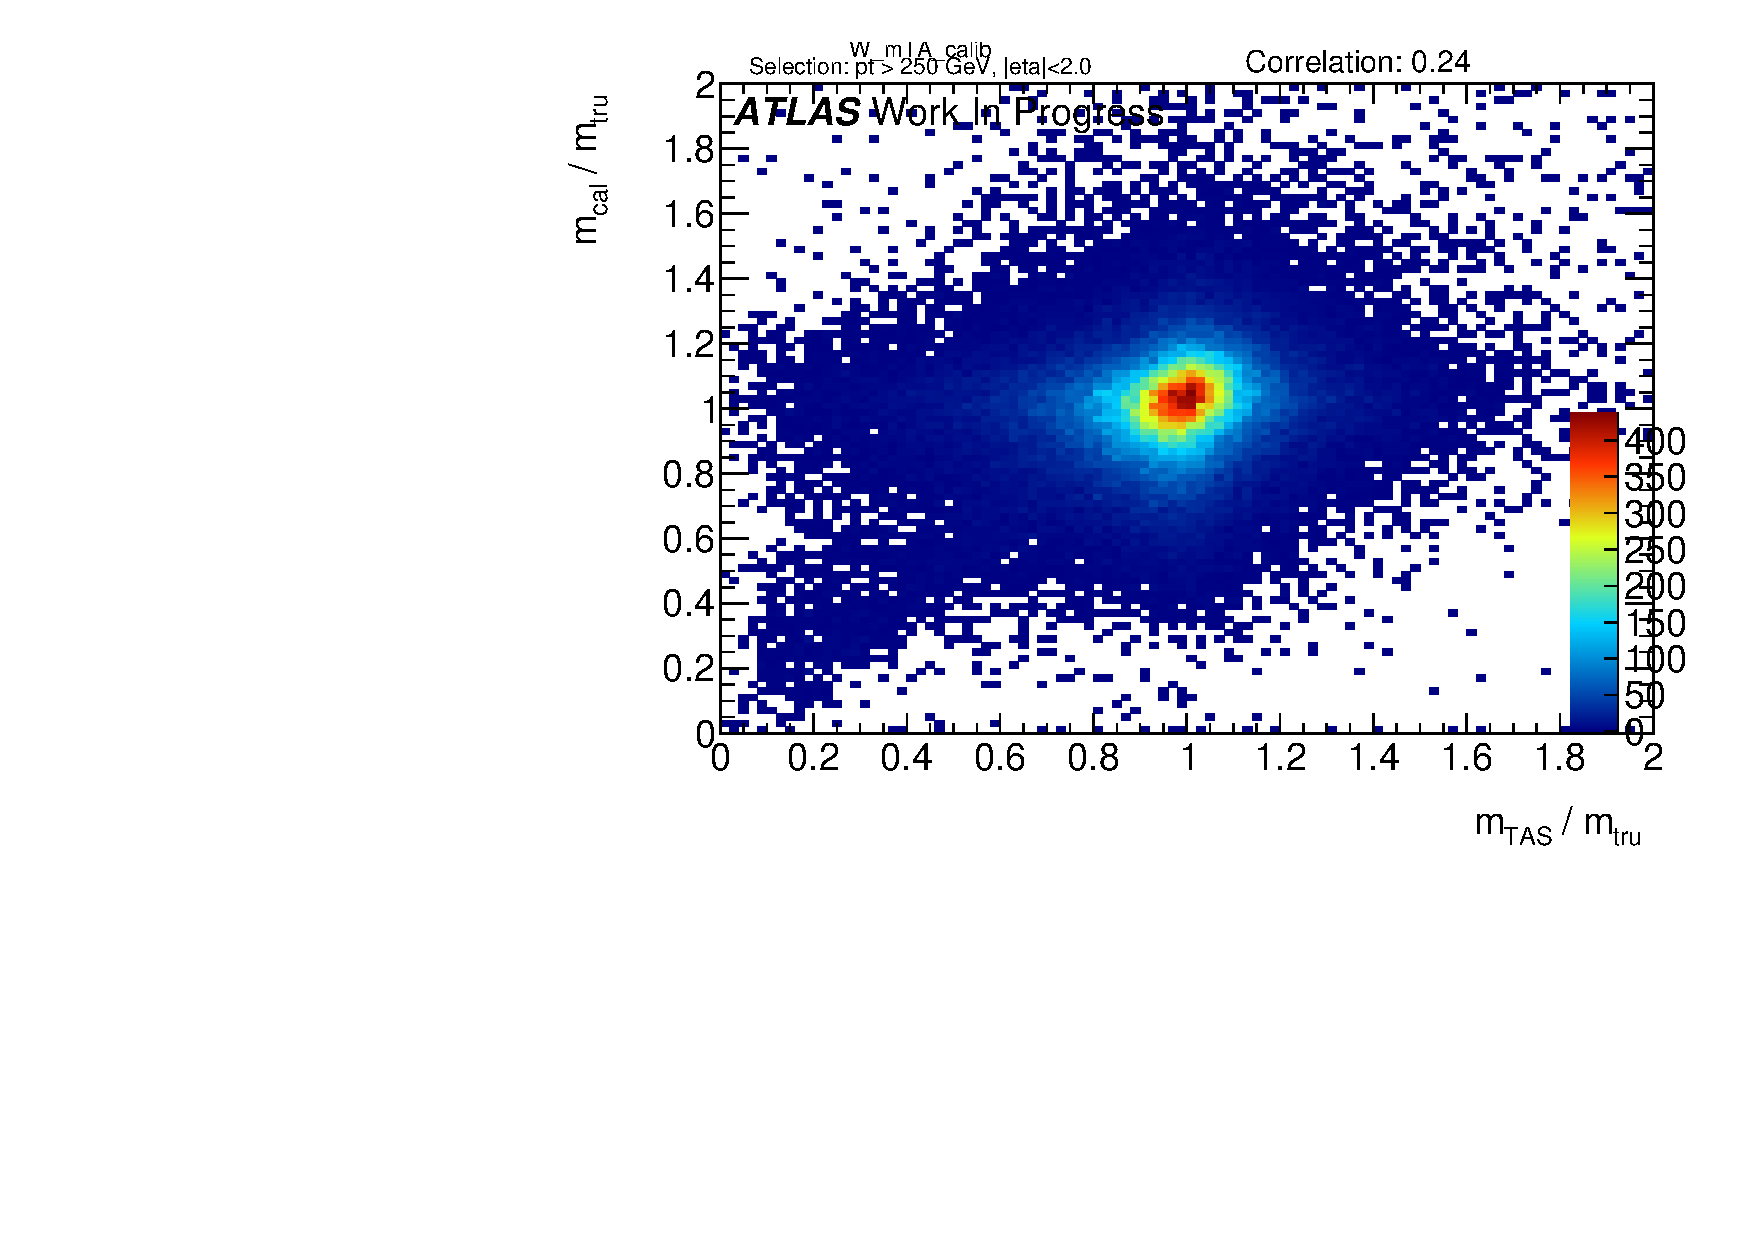
\includegraphics[width=\textwidth]{jet_part/mta/mTA_WZ/1cfrt_h_fabsca_tascal_2.pdf}
%         \rlap{\crule[white]{1cm}{1cm}}
	\put(-34,03){\crule[white]{0.15cm}{0.19cm}}
%         \label{fig:mcomba1}
    \end{subfigure}
    \begin{subfigure}[b]{0.5\textwidth}
	\centering
        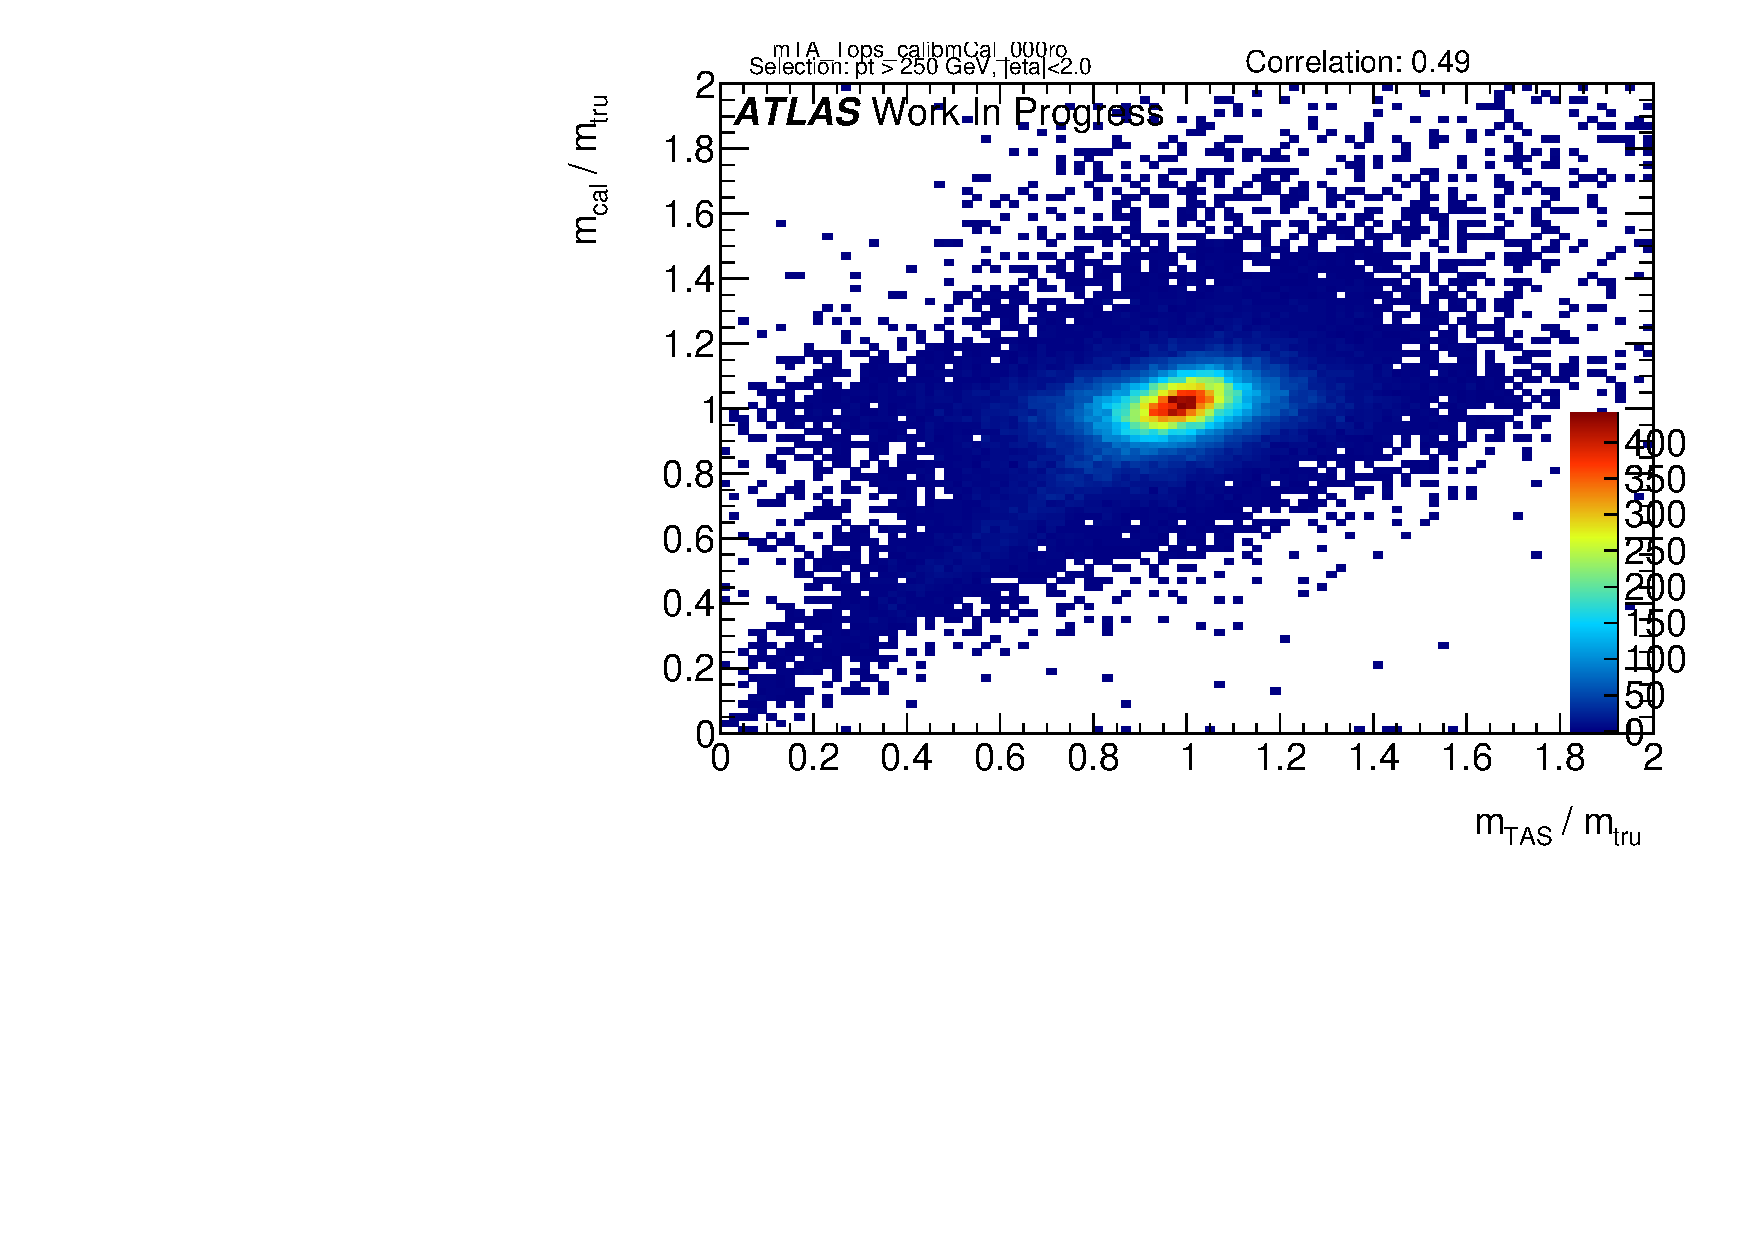
\includegraphics[width=\textwidth]{jet_part/mta/mTA_Tops/1cfrt_h_fabsca_tascal_2.pdf}
	\put(-34,03){\crule[white]{0.15cm}{0.19cm}}
%         \label{fig:mcomba2}
    \end{subfigure}
    
    \begin{subfigure}[b]{0.5\textwidth}
	\centering
        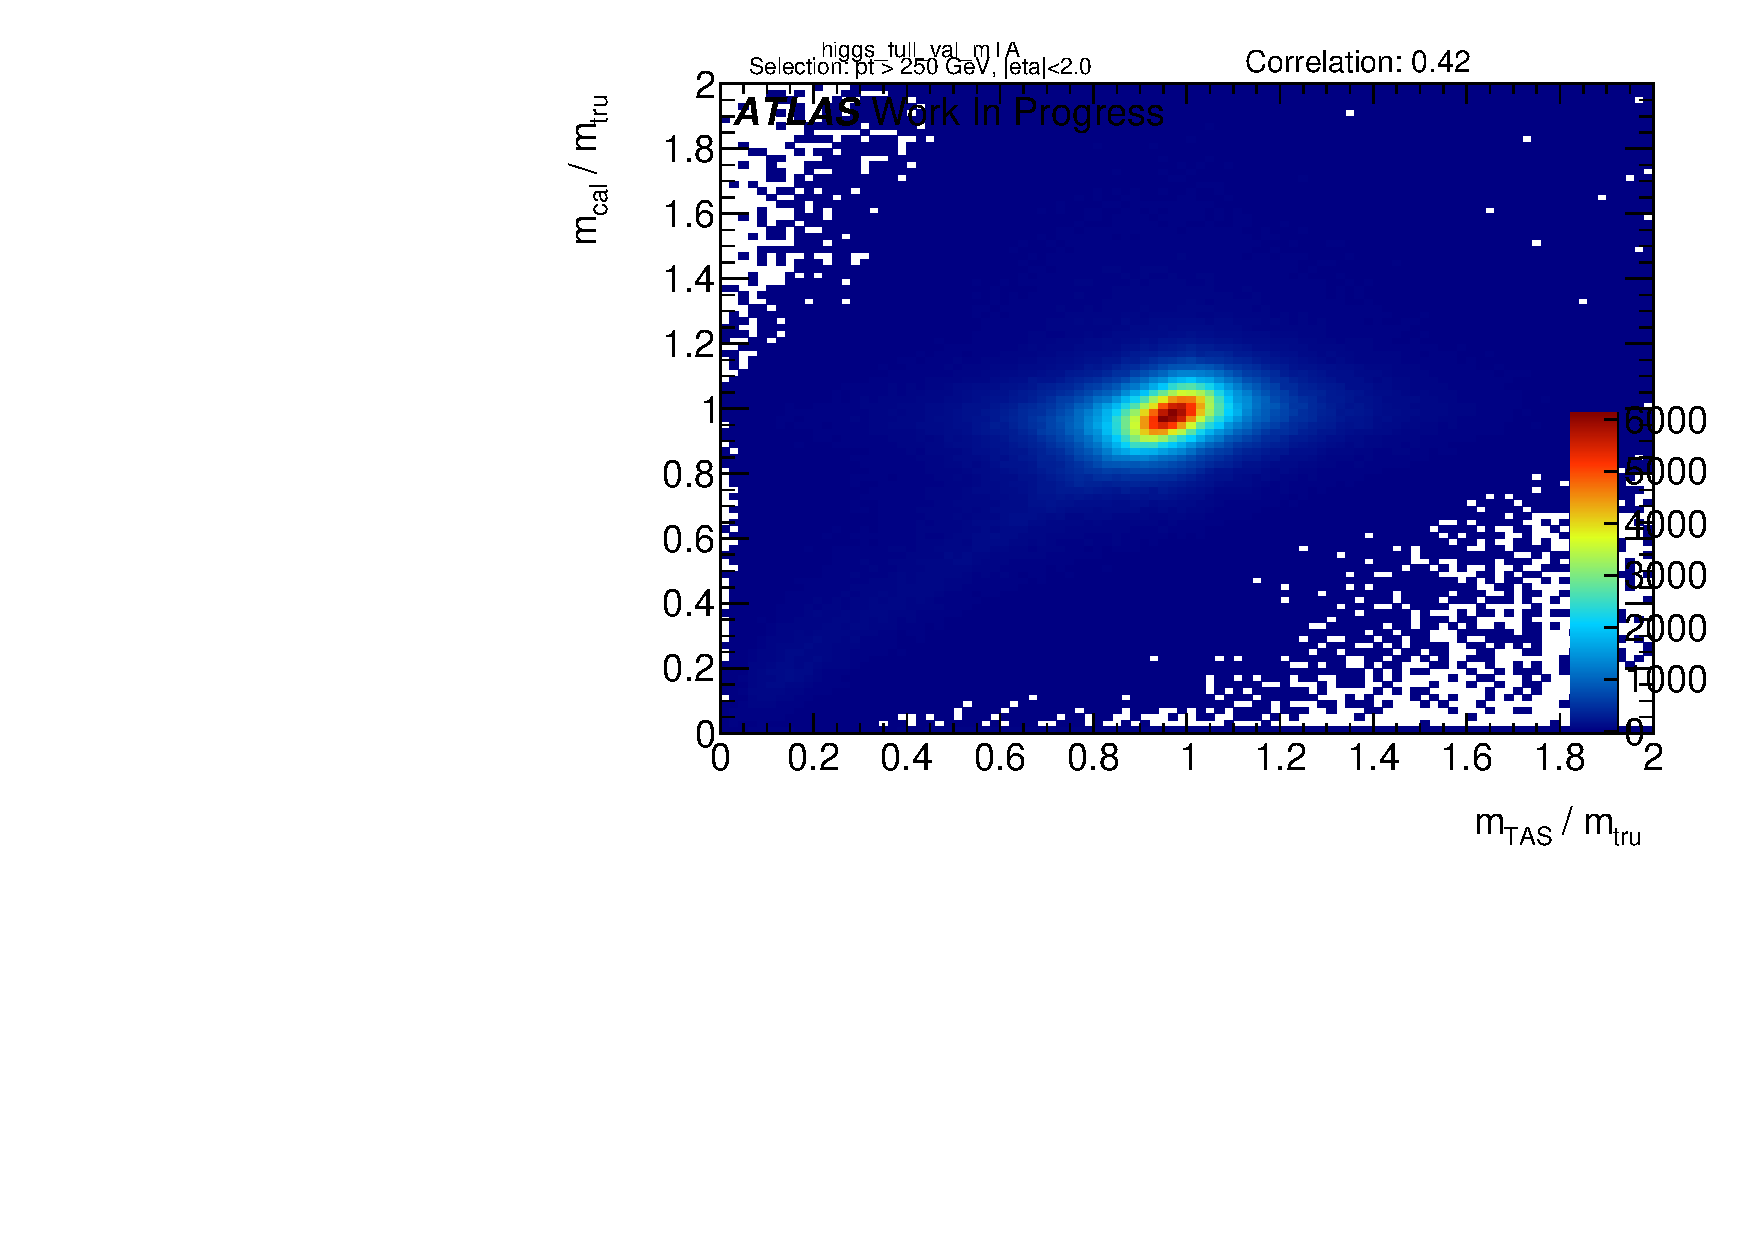
\includegraphics[width=\textwidth]{jet_part/mta/mTA_higgs/1cfrt_h_fabsca_tascal_2.pdf}
	\put(-34,03){\crule[white]{0.15cm}{0.19cm}}
%         \label{fig:mcomba3}
    \end{subfigure}
    
    \caption{Calorimeter based jet mass response vs the track-assised mass response for the three signal samples. Correlation coefficient is indicated on the top right.} 
    \label{fig:mcomba1}
\end{figure}


\begin{figure}
    \centering
   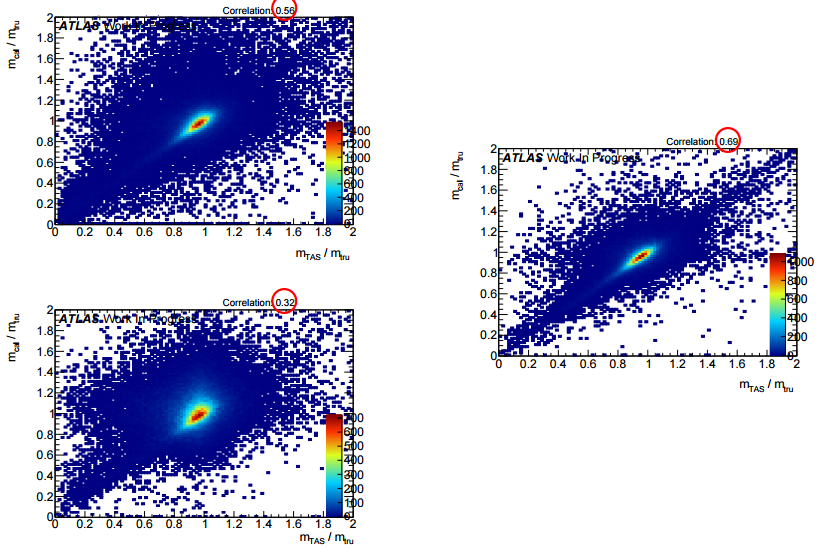
\includegraphics[width=1.2\textwidth]{jet_part/mcomb/mcomba2.png}
    \caption{Calorimeter based jet mass response vs the track-assised sub-jet mass response for the three signal samples. Correlation coefficient is indicated on the top right and highlighted.
    On the left, top, the higgs sample, bottom, the $W/Z$; on the right the top-quark sample.}
    \label{fig:mcomba2}
\end{figure}


\begin{figure}[!ht]
  \centering
      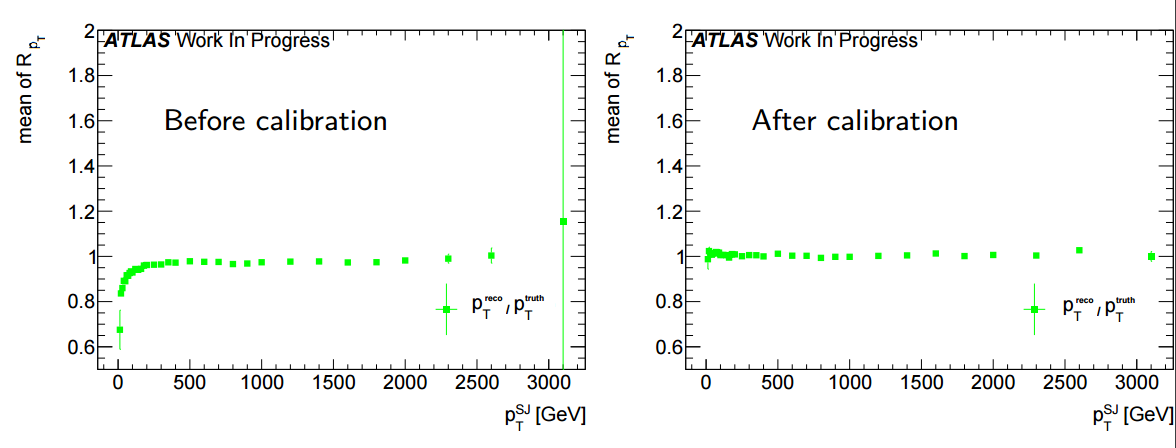
\includegraphics[width=\textwidth]{jet_part/calib/perfectcalib2.png}
  \caption{Poor's man calibration effect on mean of transverse momentum's response of the sub-jet, before, left, and after, right, the procedure.}
  \label{fig:calibA}
\end{figure}

\begin{figure}[!ht]
  \centering
      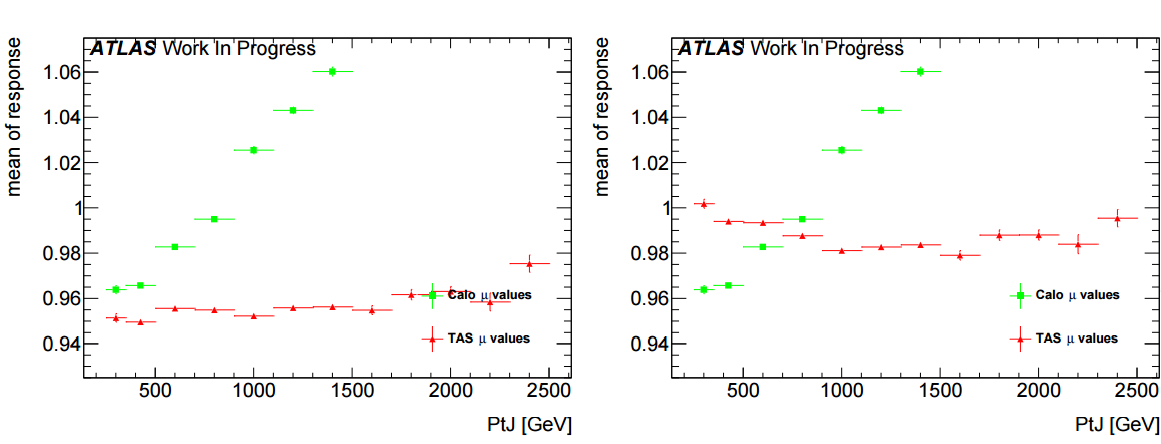
\includegraphics[width=\textwidth]{jet_part/calib/perfectcalib3.png}
  \caption{Poor's man calibration effect on the mean of the mass response of the large-R jet, before, left, and after, right, the procedure.}
  \label{fig:calibA2}
\end{figure}


\begin{figure}[!ht]
  \centering
      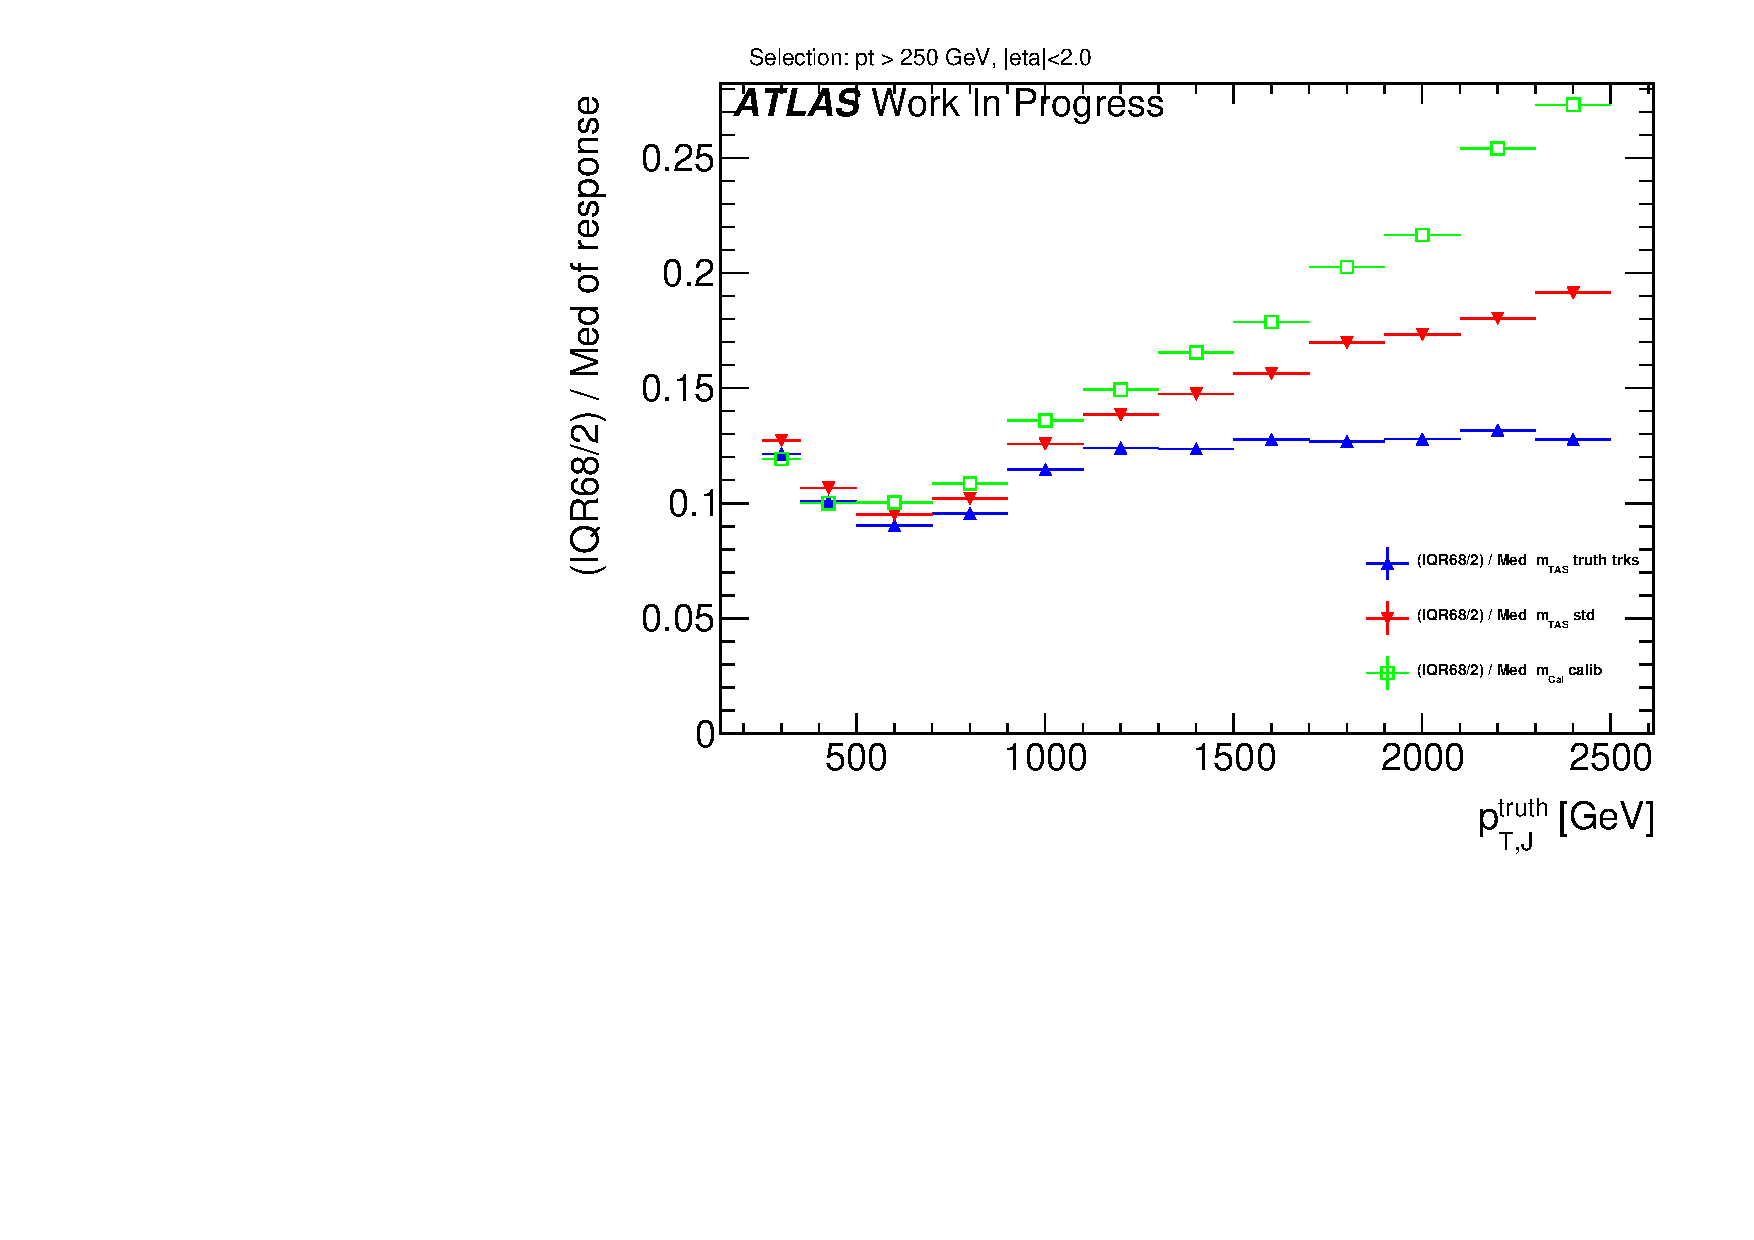
\includegraphics[width=\textwidth]{jet_part/calib/71graphcftr_h_JetRatio_mJ12CALOIQRoMcalib_degradW.pdf}
  \caption{Comparison of the $\mtas$ and the same variable using truth-level information for the tracks.}
  \label{fig:breakdown1}
\end{figure}
